%%%%%%%%%%%%%%%%%%%%%%%%%%%%%%%%%%%%%%%%%%%%%%%%%%%%%%%%%%%%%%%%%%%%%%%%%%%%

%%%%%%%%%%%%%%%%%%%%%%%%%%%%%%%%%%%%%%%%%%%%%%%%%%%%%%%%%%%%%%%%%%%%%%%%%%%%
\documentclass[12pt]{article}  % <--- 12pt font
%\usepackage[margin=1in]{geometry}% <--- 1 in margin
\usepackage[papersize={8.5in,11in},margin=1in]{geometry}
\usepackage{fancyhdr}
\pagestyle{fancy}
\fancyhf{}
\renewcommand{\headrulewidth}{0pt}
%\fancyhead[RE]{\leftmark}
\fancyfoot[LO,LE]{\tiny \emph{Conference on Information Systems and Technology, Seattle, WA, 2024}}
\fancyfoot[RO,LE]{\thepage}



\usepackage{setspace}
\usepackage{times} % <--- times new roman
%\singlespacing
\doublespace  
%%\OneAndAHalfSpacedXII % Current default line spacing
%%\DoubleSpacedXII
%%\DoubleSpacedXI

% If hyperref is used, dvi-to-ps driver of choice must be declared as
%  an additional option to the \documentclass. For example
%\documentclass[dvips,mnsc]{informs3}   % if dvips is used
%\documentclass[dvipsone,mnsc]{informs3}  % if dvipsone is used, etc.

% Private macros here (check that there is no clash with the style)
\usepackage{lscape}
\usepackage{booktabs}
\usepackage{tabu}
\usepackage{colortbl}
\usepackage{array}
\usepackage{multirow,calc,amsmath}
\newlength\mylenA
\newlength\mylenB
\newlength\mylenC
\newlength\mylenD
\usepackage{tikz}
\usepackage{tcolorbox}
\usepackage{etoolbox}
\usepackage{tcolorbox}{\normalsize}


\usepackage{adjustbox}[valign=t]

\tcbuselibrary{skins, breakable}

\makeatletter
\tcbset{
 tabular/.style={
  boxsep=\z@,top=\z@,bottom=\z@,leftupper=\z@,rightupper=\z@,
  toptitle=1anbottomtitle=1mm,boxrule=0.5mm,
  fontupper=\small,
  before upper={\arrayrulecolor{tcbcolframe}\def\arraystretch{1.1}%
   \tcb@hack@currenvir\tabular{#1}},
  after upper=\endtabular\arrayrulecolor{black}},
}
\makeatother

\usepackage{color, colortbl}
\usepackage{graphicx}
%\usepackage{subfigure}
\usepackage{caption}
\usepackage{subcaption}
%\usepackage{tcolorbox}

\usepackage{amsmath}
\usepackage{amsthm}
\usepackage{amsfonts}
\usepackage{dsfont}
\usepackage{statmath}
\usepackage{mathtools}
\usepackage{physics}

\usepackage{hyperref}
\usepackage{makecell}


% CHECK THAT THIS IS ALLOWED
\usepackage[subtle]{savetrees}

 
\newcommand{\bx}{\mathbf{x}}
\newcommand{\mD}{\mathcal{D}}
\newcommand{\mG}{\mathcal{G}}
\newcommand{\mM}{\mathcal{M}}
\newcommand{\mE}{\mathcal{E}}
\newcommand{\gray}{\rowcolor[gray]{.90}}
% Natbib setup for author-year style
\usepackage{natbib}
 \bibpunct[, ]{(}{)}{,}{a}{}{,}%
 \def\bibfont{\small}%
 \def\bibsep{\smallskipamount}%
 \def\bibhang{24pt}%
 \def\newblock{\ }%
 \def\BIBand{and}%
\def\pipeline{Explanation Pipeline}
\newcommand{\tw}[1]{\textcolor{red}{Tong: #1}}

\def\checkmark{\tikz\fill[scale=0.4](0,.35) -- (.25,0) -- (1,.7) -- (.25,.15) -- cycle;} 

\newtheorem{theorem}{Theorem}

% %%%%%%%%%%%for copyright notice
% \def\ps@IEEEtitlepagestyle{%
%   \def\@oddfoot{\mycopyrightnotice}%
%   \def\@evenfoot{}%
% }
% \def\mycopyrightnotice{%
%   {\footnotesize 978-1-4799-6773-5/14/\$31.00 \textcopyright2017 Crown\hfill}
%   \gdef\mycopyrightnotice{}
% }
% %%%%%%%%%%%

% \let\old@ps@headings\ps@headings
% \let\old@ps@IEEEtitlepagestyle\ps@IEEEtitlepagestyle
% \def\confheader#1{%
%   % for all pages except the first
%   \def\ps@headings{%
%     \old@ps@headings%
%     \def\@oddhead{\strut\hfill#1\hfill\strut}%
%     \def\@evenhead{\strut\hfill#1\hfill\strut}%
%   }%
%   % for the first page
%   \def\ps@IEEEtitlepagestyle{%
%     \old@ps@IEEEtitlepagestyle%
%     \def\@oddhead{\strut\hfill#1\hfill\strut}%
%     \def\@evenhead{\strut\hfill#1\hfill\strut}%
%   }%
%   \ps@headings%
% }
% \makeatother

% \confheader{%
%     \tiny
%     \parbox{20cm}{Workshop on Information Technology and Systems, Hyderabad, India 2023}
% }

%% Setup of theorem styles. Outcomment only one.
%% Preferred default is the first option.
%\TheoremsNumberedThrough   % Preferred (Theorem 1, Lemma 1, Theorem 2)
%\TheoremsNumberedByChapter % (Theorem 1.1, Lema 1.1, Theorem 1.2)
%\ECRepeatTheorems

%% Setup of the equation numbering system. Outcomment only one.
%% Preferred default is the first option.
%\EquationsNumberedThrough  % Default: (1), (2), ...
%\EquationsNumberedBySection % (1.1), (1.2), ...

% For new submissions, leave this number blank.
% For revisions, input the manuscript number assigned by the on-line
% system along with a suffix ".Rx" where x is the revision number.
\date{}
%%%%%%%%%%%%%%%%
\begin{document}

\title{The Risk of Inferring Data Insights from Post Hoc Explanations of Machine Learning Models}

\author{Anonymous Authors\footnote{Best Student Paper Award consideration: the bulk of this work was done by a student author.}}
%\date{April 2020}

% palette for colorblindness https://davidmathlogic.com/colorblind/#%23000000-%23E69F00-%2356B4E9-%23009E73-%23F0E442-%230072B2-%23D55E00-%23CC79A7

\maketitle

\begin{abstract}
Machine learning models have been increasingly used in business research. However, most state-of-the-art machine learning models, such as deep neural networks and XGBoost, are black-boxes in nature. Therefore, post hoc explainers that provide explanations for machine learning models such as feature importance, have been gaining wide usage. Despite the intended use of the post hoc explainers being explaining machine learning models' predictions, we found a rising trend in business research where post hoc explanations, more specifically feature importance, are used to infer \emph{how} explanatory variables ($X$) are associated with the target variable ($Y$): especially in terms of the signs and relative importances of the marginal effects of $X$ on $Y$. In this work, we investigate the validity of such use. Specifically, we investigate with extensive experiments \emph{whether} the feature importance obtained by the two most popular post hoc explainers, SHAP and LIME, provide correct information about the true marginal effect of $X$ on $Y$ in the \textit{data}, a property we refer to as data-alignment. We then identify \emph{what} factors influence the alignment of explanations. Finally, we propose a set of mitigation strategies to improve explanations and demonstrate their effectiveness with real-world data in an econometric context. In spite of this effort, we nevertheless conclude that post hoc explainers should only be used to propose hypotheses on data rather than validate hypotheses. The ultimate goal of this paper is to caution business researchers \textit{against} translating explanations of machine learning \textit{models} into potentially false insights and understanding of \textit{data}. %trusting and putting into practice insights they obtain from post hoc explainers. % we investigate whether post hoc explanations contain three types of information about the marginal effects of features in data, based on recent literature. We formalize the three types of information and refer to explanations that can capture them as data-aligned. We identify factors within the explanation pipeline that are associated with explanations that are not data-aligned. We find ideal conditions where LIME explanations are data-aligned, and we show theoretically that SHAP is inherently unsuited for recovering marginal effects. We also discuss the issue of explanation inconsistency, which is due to varying choices of models, explainers, and their configurations. Furthermore, we propose simple mitigation strategies for low data-alignment and inconsistency that we encourage researchers to use as a foundation for experimentation. We validate our mitigation strategies in an econometric context and demonstrate the resulting improvement in explanation quality. Despite these efforts, we nevertheless conclude that researchers should only use post hoc explainers to infer data insights with great caution.


% Post hoc explanation methods like LIME and SHAP have become very popular for
% interpreting machine learning models. but unique problems arise when they are used in business contexts, since stakeholders may want to draw managerial insights
% based on them. In this work, we investigate how and why post hoc explanations can be misused or
% misunderstood in business research. Our investigation proceeds by diagnosing and demonstrating
% issues we identify in what we call the Prediction Insight Pipeline in business research. The pipeline
% starts with researchers building a black-box model, using a post hoc explainer to explain the model, and ends with researchers using the explanations to make inferences about their business. We demonstrate the incorrectness and inconsistency of post hoc explanations and demonstrate their consequences on managerial insights. Finally, we propose and test mitigation strategies. 
\end{abstract}%
%
%%%%%%%%%%%%%%%%%%%%%%%%%%%%%%%%%%%%%%%%%%%%%%%%%%%%%%%%%%%%%%%%%%%%%%

% RONILO: Idea for the structure of our critique
% 1. Identify the underlying assumptions and conditions for the use of post hoc explainers. e.g. it's hard to make an intrinsically interpretable model, small rashomonon set, already have good bviolin (sunk cost fallacy...)
% 2. Presuppose the conditions for post hoc explainer ot be effective. e.g. M is accurate, data satisfies causal inference conditions. What are the effects when they are and aren't satisfied?
% 3. Examine the social relations generated by post hoc explainers. In this paper we just care about those between data scientists, model builders, and ***MANAGERS***. 
% 4. Identify the contradictions and tensions within the use of post hoc explainers. e.g. multiplicity, wrong explanations, no actionable recourse, business owners misled into making harmful decisions
% 5. Evaluate the potential for mitigation strategies involving G, M, the data, and post hoc explainers both alone and together. 

\newpage

\section{Introduction}
  % Mention Marketing Science Institute "consistently identified attribution as a topmost research priority over the last few years" (from SHAP meets uniform paper)

% =========================== Tong ===========================
Over the past few decades, the surge in data volume and complexity has led to the widespread adoption of machine learning (ML) for business analysis \citep{kleinberg2015prediction,mullainathan17applied}. ML is commonly used in scenarios involving numerous variables where researchers focus on predicting a particular variable of interest. This translates into formulating a supervised learning problem where the target variable is predicted by an ML model using available features (explanatory variables).

However, in business research, prediction alone is often insufficient. Researchers and practitioners are also interested in gaining insights about the data through predictive ML models. In particular, they seek information about how explanatory variables are associated with the target variable, a relationship that can be described by the marginal effects of the explanatory variables\footnote{Note that marginal effects are descriptive and do not directly indicate causality.}.  %For example, \cite{sanchez2023role} used SHAP explanations of an ML model to try to understand what drives hotel guest satisfaction and made service strategy recommendations for hotel managers on the basis of the SHAP explanations. 
Unfortunately, most ML models with high accuracy operate as black boxes \footnote{It is worth acknowledging that recent years have seen the emergence of inherently interpretable models that can attain comparable performance to black box models, sans the reliance on post hoc explanations. However, these models, which lie beyond the purview of this paper's discussion, will not be further delved into here.} that produce predictions without providing any insight into their internals. This gives rise to a new type of method, called post hoc explainers, which provide various types of explanation of black-box models, such as feature importance \citep{ribeiro16lime,lundberg17shap}, partial dependence plots \citep{friedman01pdp}, counterfactual examples \citep{mothilal20dice}, etc. %This prompts researchers to seek ways to get data insights from predictive models. 
 Many recent business research efforts follow what we call the Explanation Pipeline in this paper, shown in Figure \ref{fig:pipeline}. %, where a black-box ML model is employed for a complex prediction task and subsequently explained by a post hoc explainer. 
 An explanation pipeline consists of two stages. First, a machine learning model, which we denote by $\mathcal{M}$, is trained on data $\mathcal{D}$. We call this the \emph{prediction stage}. Then in the second stage, the \emph{explanation stage}, an explainer model (e.g. LIME or SHAP), denoted by $\mathcal{E}$, is applied to $\mathcal{M}$ to generate explanations of $\mathcal{M}$. %We use $e_{\mE}(x^{(i)}_j)$ to represent the explanation (i.e., feature importance) for feature $X_j$ in the $i^{\text{th}}$ data instance $\mathbf{x}^{(i)}$. We call the production of the $e_{\mE}(x^{(i)}_j)$ the \emph{explanation stage}. %%This expectation is particularly pertinent for explainers that produce feature importance, such as LIME \citep{ribeiro16lime} and SHAP \citep{lundberg17shap}\footnote{We will only study SHAP and LIME in this paper.}.

Post hoc explanations are meant to provide insight into the decision-making process of ML models. However, a growing number of recent papers consider it natural to expect that these explanations can also be extrapolated to understand data. 
Indeed, recent literature increasingly adopts this perspective. SHAP and LIME explanations of black box models have been extrapolated in diverse areas of business literature to make inferences about the marginal effects of the features. We meticulously examined 150 papers from the business literature utilizing either SHAP or LIME, spanning from 2018\footnote{LIME was published in 2016, and SHAP was published in 2017. Considering the time it takes to write a business paper, we set the start time of our literature search to 2018 for papers that use either LIME or SHAP.} to 2024. Notably, our findings reveal that among these 150 papers (109 of which are from top journals \footnote{We consider a journal a top journal if the 5-year impact factor is above 5 or the journal is an INFORMS journal. Note that SHAP and LIME are relatively new methods, and the business journal review processes are long. Therefore, many papers are still under review and are not counted among the 109 top journal papers we reviewed.}), 42\% used explanations to draw conclusions on the $X$ and $Y$ relationship in the data, rather than in the model. For instance, \cite{park2024extracting} claimed that SHAP explanations provide guidance on what smartphone features customers prefer, and \cite{jiang24churn} says that if a customer has a large value for a feature that often has large SHAP values, they are more likely to be churners. Some recent work is quite optimistic about post hoc explanations; \citep{berger2023supply} advocate the use of the combination of an ML model and SHAP as an ``alternative to OLS''.

Such use of explainers to draw conclusions on data suggests an emerging paradigm shift in which, through post hoc explanations, ML models are used not only for prediction but also as a means to gain understanding of data. However, the validity of using explainers for this purpose remains unjustified. 

Therefore, the goal of this paper is to conduct a thorough investigation into this new and emerging trend of research methodology so that we might advise the business research community
against this particular inappropriate use of post hoc explainers. We aim to directly answer the question, %``\emph{Can explanations from SHAP and LIME be extrapolated to infer $X$ and $Y$ relationship in the data?}''
``\emph{Can SHAP and LIME explanations capture the correct relationship between $X$ and $Y$, specifically the marginal effect of $X$ on $Y$, in the data?}''
with both empirical and theoretical evidence. Additionally, we use the results of our analyses to propose some mitigation strategies to improve SHAP and LIME explanations. We show that these strategies help to improve the alignment of SHAP and LIME with results from a real econometric study on loan approval, but cannot fully eliminate the causes of misaligned explanations.

Overall, our paper identifies and cautions against a growing trend of the inappropriate use of post hoc explanations to draw definite conclusions on data. We argue that post hoc explanations should not be used to \textbf{validate} hypotheses about data; instead, their role in gathering knowledge about data should be limited to \textbf{proposal} of hypotheses. To gain an accurate understanding of the underlying relationships between $X$ and $Y$ in the data, we emphasize the need for more rigorous and comprehensive follow-up analyzes, both quantitatively and qualitatively. This distinction is essential to ensure the prevention of the overestimation of the reliability and validity of insights derived from machine learning models in business research.

The paper is organized as follows. %We will review related work in Section \ref{sec:related_work}. 
We introduce a simulated data generation process and ground truth model for loan approval that we will use to benchmark the data-alignment of SHAP and LIME. We provide theoretical and empirical analyses on why post hoc explanations are not suitable to infer information about marginal effects in Section \ref{sec:misalignment}. We then explore some mitigation strategies for SHAP and LIME in Section \ref{sec:mitigation_strategies} by gauging how beneficial they are over baselines in reproducing the findings of an econometric study on real loan application data. The paper concludes in Section \ref{sec:discussion} with a summary of our findings and final remarks on post hoc explanations and their use in business research. %%In the Appendix, we corroborate all of the experiments in the main body of the paper by running them a second time using a synthetic direct marketing dataset. 
  


% \section{Related Work}
%   \label{sec:related_work}
%  % This section introduces LIME and SHAP and then gives a review of prior literature discussing their weaknesses. We summarize some theoretical and practical issues they have.
  
%   LIME and SHAP are model agnostic attributive post hoc explainers which estimate a feature importance for each feature without accessing the internals of the models, and henceforth ``model agnostic". LIME's feature importance values are coefficients from the underlying linear surrogate models, which are solutions to synthetic regression problems using sampled data around the point being explained. SHAP's surrogate model is special in that its coefficients represent Shapley values \citep{shapley97shapley}, originally used in game theory to allocate fair shares of a valuable quantity to the individuals who cooperated in obtaining it. 
%   Post hoc explainers aim to help humans understand black box models, but their current designs are often not conducive to that goal. Most importantly, their explanations are generally erroneous \citep{rahnama19shift,kumar20shap}. For example, they may not give importance to important features \citep{garreau20theoretical}. Secondarily, they are prone to giving inconsistent explanations that may cause confusion \citep{Barocas20assumptions,bansal20sam,molnar2019,alvarez18robustness,laugel18defining,artelt21evaluating}.

\vspace{-3mm}
\section{Data Generation}
\label{sec:data_generation}\vspace{-3mm}
We will analyze the Explanation Pipeline using a simulated loan approval dataset for a running example\footnote{We use simulated data for the experiments because we require access to the ground truth in order to compare the post hoc explanations with the ground truth.}. The dataset is designed to model the task of predicting whether an individual will be approved for a loan based on their demographic and credit-related features. We define a linear model for generating the dependent variable such that the ground truth is known and controllable. The linearity of the ground truth also makes the explanation task relatively easier for the explainers. The ground truth, as well as the features used to construct it, are designed as follows.


 % \paragraph{Data Generation Process}
 % \label{sec:data_generation}
 % \paragraph{Data Generator $\mathcal{G}$}
 %In this section, we will introduce a simulated dataset, variants of which will be used throughout the paper. 
 % thus the coefficients in the linear model are used for the ground truth. %The ground truth model is linear, so we can evaluate local explanations with respect to the ground truth's global explanation. 
We first generate the features. Each data point represents an applicant with ten features: four demographic features and six credit-related features. Table \ref{tab:simulated} summarizes how each feature is generated. % We also include an unobserved confounder to enhance the realism of the dataset - this feature is used to generate the label but not observed by $\mathcal{M}$. % The meanings and manners of construction of all the features are reported in Table \ref{tab:simulated}. 
Among those, the credit score feature is generated based on a partial FICO credit scoring model \citep{ligons_fico} and is calculated as: $\text{Credit score}= 650 + (10 + 2.5\cdot \text{Credit history}) + (70 - 15 \cdot \text{Inquiries}) + (35 - 4 \cdot \text{Delinquencies}) + (105 - 100 \cdot \text{Utilization})$. ``Cosigner" is positively correlated with ''Married: in that the probability of having a cosigner is given by $\sigma(2\cdot \text{Married} + 1 + \epsilon)$ where $\epsilon \sim \mathcal{N}(0,\frac{1}{2})$. 
% % feature description table
% \begin{table}[h]
% \centering
% %\resizebox{\textwidth}{!}{%
% \footnotesize
% \begin{tabular}{c|c|c}
% \toprule
% \textsc{Feature} & \textsc{Explanation}              & \textsc{Formula}    \\ \toprule
% Age       & Applicant Age                  & Uniform(18,100)    \\ 
% Sex       & Applicant Sex                  & Bernoulli(.5)     \\
% Married     & Applicant Marital Status            & Bernoulli(.5)     \\ 
% Income      & Applicant Income                & Normal(40,000, 30,000) \\ 
% Inquiries    & Number of credit inquiries           & Uniform(0,6)      \\ 
% Cosigner     & Indicator of presence of loan cosigner & Function of marital status     \\ 
% Utilization   & Proportion of total credit utilized      & Uniform(0,1)      \\ 
% Delinquencies  & Number of delinquent payments in last 2 years & Uniform(0,24)     \\ 
% Credit Score   & Credit score based on FICO scoring & FICO credit scoring model \citep{ligons_fico}      \\ \bottomrule
% \end{tabular}%
% %}
% \caption{Description of features for simulated loan data.}
% \label{tab:simulated}
% \end{table}

  We then define a ground truth model $\mathcal{G}$ for generating applicants' labels, \textit{approved}, or \textit{rejected}. This ground truth model represents the real-world decision-making process that is never observed. Therefore, for the purpose of demonstration, we define $\mathcal{G}$ so that we can directly compare the explanations with the ground truth. We define $\mathcal{G}$ as a linear model and then compose it with a logistic sigmoid function to generate the labels. The true marginal effects $\boldsymbol{\beta}$ are defined using the coefficients of $\mathcal{G}$\footnote{The coefficients $\mathcal{G}$ can differ from $\boldsymbol{\beta}$ because we define the $\beta_j$ for a feature which influences other features to be the total derivative of the response with respect to that feature.}; it is the ground truth we compare the feature importance values provided by SHAP and LIME against. $\mathcal{G}$ is defined as the following linear model taking standardized features as input. 
  % \textcolor{red}{$\mathcal{G}$ has to use all features somewhere in the paper, if not section 3 then section 4 and 5 for demonstrating some issues. If there are features in Table 2 not used by G ever, remove it}
  %\begin{tcolorbox}%[title = Ground Truth Model $\mathcal{G}$]
  \vspace{-2mm}
  \begin{equation}
  \label{eqn:gt}
  \begin{split}
  \mathcal{G}(X) =2.5 +.0005\cdot\text{Age} -0\cdot\text{Sex} +.1 \cdot \text{Married} + .25\cdot \text{Cosigner} + 1.5 \cdot \text{Credit History} + \\  3 \cdot \text{Income} - 1\cdot\text{Utilization} -.75 \cdot \text{Delinquencies} - .5\cdot\text{Inquiries} + 5.\cdot\text{Credit Score} + \epsilon
  \end{split}
  \end{equation} \vspace{-2mm}
  %\end{tcolorbox}
  \noindent where $\epsilon \sim \mathcal{N}(0,\frac{1}{4})$ captures all the variation in the response variable that is not explained by the explanatory variables.
  Using the logistic sigmoid function $\sigma(\cdot)$, we assign $Y = 1$ (approved) for cases with $\sigma(\mathcal{G}(\mathbf{x}))\geq 0.5$, and $Y = 0$ (rejected) otherwise. The intercept term 2.5 is chosen so that, at a baseline, when feature values are zero (as the features are standardized, the means of numerical features are zero), an applicant is most likely accepted. %The remaining coefficients are chosen so that credit score is the most important feature, followed by credit inquiries, delinquencies, income, credit history, marital status, cosigner availability, marital status, age, and finally sex. 
  The coefficient values used in $\mathcal{G}$ are motivated by empirical facts from the literature \cite{cfb_age, Calcagnini2014}. %the following empirical facts. The probability of being approved for a loan increases insignificantly with age \citep{cfb_age}, but significantly with credit score. The probability decreases significantly as applicants use higher proportions of their available credit and receive recent credit inquiries. The sex of a customer is not supposed to affect approval outcomes~\citep{Calcagnini2014}.

  Therefore, we create a dataset $\mathcal{D}$ with 5000 data points by sampling from the distributions of features to simulate applicant profiles ($\mathbf{x}$) and using $\mathcal{G}$ to create the labels ($Y$). 
  %%In the following, we apply the Explanation Pipeline to demonstrate how one obtains an understanding of marginal effects by explaining $\mathcal{M}$ using $\mathcal{E}$. %Our demonstration will motivate the subsequent sections of the paper, which focus on investigating and mitigating unfaithful and inconsistent explanations.

\vspace{-3mm}
\section{Misalignment of Post Hoc Explanations}
  \label{sec:misalignment}\vspace{-3mm}
  In this section, we study a most important question: Do post hoc explanations of a model $\mathcal{M}$ provide correct information about the true marginal effects of features in $\mathcal{G}$? We first describe how we evaluate explanations in Section \ref{sec:evaluating_faithfulness}. 
  Then, in Section \ref{sec:causes_of_misalignment}, we identify properties of the data $\mD$, the model $\mM$, and the explainer $\mE$ used in a pipeline that lead to misaligned explanations and demonstrate how those individually affect the explanation. Finally, we adduce the generality of the problem of misalignment in Section \ref{sec:pervasive}. %%The experiments in this section all use our running example of explaining loan application decisions, where the ground truth model is a linear model. 

\vspace{-2mm}\subsection{Assessing the Data-Alignment of Explanations}
  \label{sec:evaluating_faithfulness}\vspace{-2mm}
  Both SHAP and LIME provide a feature importance for each feature $j$, denoted by $e_\mE(x^{(i)}_j)$, where $\mE$ represents the explainer. 
   Our goal is to investigate whether $e_\mE(x^{(i)}_j)$ can be used to provide correct information about the marginal effect of feature $j$, in terms of three different aspects motivated by practical use cases of explanations from the literature: the sign, the importance ranking, and relevance. 

We define three metrics to represent these relevant aspects of the ground truth.
  The first metric, termed \textbf{directionality}, measures whether post hoc explainers can at least identify the correct \textit{sign} of a feature's influence on the outcome. It evaluates an explanation only qualitatively. We calculate directionality by determining the percentage of cases where the sign of $e_\mE(x^{(i)}_j)$ matches that of $\beta_j$ for each feature $j$ across $m$ instances in the test set. 
  % \begin{equation}
  %   \label{eq:acc}
  %   \texttt{directionality}(\{e_\mE(x^{(i)}_j)\}_{i=1}^m,\beta_j) = \frac{1}{m} \sum_{i=1}^m s_j( e_\mE(x^{(i)}_j),\beta_j)
  % \end{equation}
  % where 
  % \begin{equation*}
  %   s_j(e_\mE(x^{(i)}_j),\beta_j) = \begin{cases*}
  %         \mathbf{1}_{\mathbb{R}^+}(\beta_j \cdot e_\mE(x^{(i)}_j)) & if $\mid \beta_j\mid > \epsilon_1$ \\
  %         \mathbf{1}_{(0,\epsilon_2)}\left(\frac{\mid e_\mE(x^{(i)}_j)\mid }{\max_{j'} \mid e_\mE(x^{(i)}_{j'})\mid}\right) & otherwise
  %       \end{cases*}
  % \end{equation*}
  % Here $\mathbf{1}_S(z)$ is an indicator function that returns 1 if $z\in S$ and outputs 0 otherwise. $s_j(e_\mE(x^{(i)}_j),\beta_j)$ is designed to facilitate a relaxed version of accuracy by checking if $\beta_j$ and $e_\mE(x^{(i)}_j)$ have the same sign only when $\beta_j$ is not very small, i.e. larger than $\epsilon_1$. When $\beta_j$ is small, $s_j$ instead checks if $e_\mE(x^{(i)}_j)$ is small relative to the other $e_\mE(x^{(i)}_{j^{\prime}})$, $j\prime \neq j$. The ratio of $\mid e_\mE(x^{(i)}_j)\mid $ and $\max_j^\prime \mid e_\mE(x^{(i)}_{j^\prime})\mid$ should be small, i.e. at most $\epsilon_2$.
  % In our experiments, we use $\epsilon_1=1e-2$ and $\epsilon_2=1e-2$. 
  The second metric, \textbf{concordance}, measures how accurately the explanations recover the \textit{relative importance} of features compared to the ground truth, $\beta_j$. Given the $e_\mathcal{E}(x^{(i)}_j)$, we rank the features from least to most important and calculate the \emph{Spearman Rank Correlation} \cite{spearman1904proof} between this ranking and a ranking of the $\beta_j$.
  %%While the directionality metric is computed using the entire test set per feature, the concordance is computed per instance using all features.
  % % The Spearman rank correlation is defined as follows. 
  % \begin{equation}
  %  \texttt{concordance}(e_\mE(\mathbf{x}^{(i)}),\boldsymbol{\beta}) = 1 - \frac{6\sum_{j=1}^d (\text{rank}(\beta_j) - \text{rank}(e_\mE(x^{(i)}_j)))^2}{d(d^2-1)},
  % \end{equation}
  % where $d$ is the number of features, and $\text{rank}(\beta_j)$ and $\text{rank}(e_\mE(x^{(i)}_j))$ denote the rank of the $j^{\text{th}}$ feature according to the coefficients of $\boldsymbol{\beta}$ and explanations $e_\mE(\mathbf{x}^{(i)})$, respectively. 
  %%If the explainers' rankings are 100\% correct, then the correlation should be 1. Any value less than 1 indicates an error in the rankings, leading users to misinterpret the importance of some features.
  Third, motivated by the fact that researchers may only be interested in identifying a small set of features that have the biggest impact, we define the third metric, \textbf{relevance}, based on the ranking of features. Our metric, denoted $\text{relevance}_k$, measures how many of the top-$k$ most important features identified by $\mathcal{E}$ are indeed among the top-$k$ largest (in magnitude) marginal effects. These three metrics capture three primary types of information sought by researchers in emerging business literature. We refer to high performance of an explainer with respect to these metrics as \textbf{alignment} with the data.
  % Denote by $I_k^+(e_\mE(\mathbf{x}^{(i)}))$ and $I_k^+(\boldsymbol{\beta})$ the set of feature indices among the top-$k$ most highly ranked according to $e_\mE(\mathbf{x}^{(i)})$ and $\boldsymbol{\beta}$, respectively. Then we define 
  %   \begin{equation}
  %     \texttt{relevance}_k(e_\mE(\mathbf{x}^{(i)}), \boldsymbol{\beta}) = \frac{\mid I_k^+(\boldsymbol{\beta}) \cap I_k^+(e_\mE(\mathbf{x}^{(i)}))\mid}{k}.
  %   \end{equation}
     %%Like the concordance metric, $\text{relevance}_k$ is also computed at the instance level. 
    %%In our experiments, we compute $\text{relevance}_k$ for each $k$ and plot the means and standard errors over $m$ instances. $\text{relevance}_k(e_\mE(\mathbf{x}^{(i)}), \boldsymbol{\beta})$ represents the true positive rate for the identification of what features are among the top-$k$ largest marginal effects according to $\mathcal{E}$.    
  
  
    




 %%\paragraph{Data-Alignment Evaluation}
 %% We call the evaluation of the directionality, concordance, and relevance the evaluation of \textbf{data-alignment}. We evaluate the data-alignment for SHAP and LIME on $m=100$ applicants randomly selected from the test set and report the results in Figure \ref{fig:beta_alignment}. We find that neither SHAP or LIME achieves satisfying results on any of the three dimensions. Particularly, SHAP, while strongly favored over LIME by researchers, perform significantly worse than LIME in all three dimensions. SHAP cannot even identify the correct directionality of the features, let alone the concordance. To have a better understanding of SHAP, we also simulate a \emph{random} explainer that randomly draws its feature importance values $e_\text{random}(x^{(i)}_j)$ from a standard normal distribution for each $j$ and $i$. We find that \emph{SHAP explanations do not have better data-alignment than random explanations do with respect to directionality and concordance.}     
    %       \begin{figure}[ht!]
    %   \centering
    %   \begin{subfigure}[t]{.2\textwidth}
    %    \centering
    %    \captionsetup{justification=centering}
    %      \raisebox{.2cm}{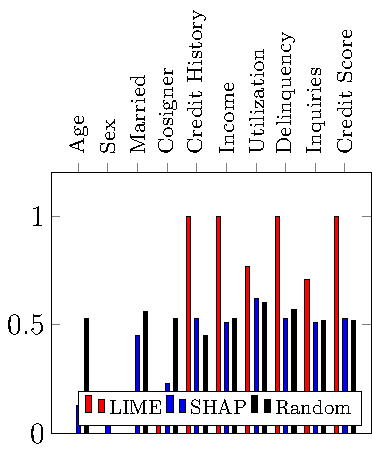
\includegraphics[width=\textwidth]{Figs/sec4_1-figure0.pdf}}%{Figures/lime_shap_Spearman_magnitude.png}

    %    \caption{Directionality}%Spearman rank correlations of feature importance magnitudes from SHAP and LIME against the true ranking from $\mathcal{G}$. }
    %    \label{fig:lime_shap_sign_accs}
    %   \end{subfigure}%
    %   \hspace{1cm}%\hfill
    %   \begin{subfigure}[t]{.2\textwidth}
    %    \centering
    %    \captionsetup{justification=centering}
    %    \raisebox{.05cm}{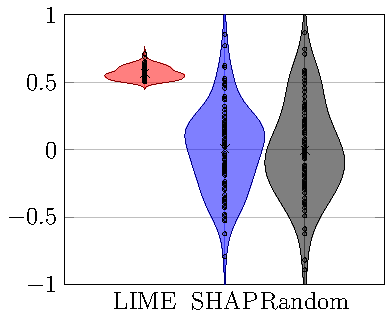
\includegraphics[width=\textwidth]{Figs/sec4_1-figure1.pdf}}%{Figures/lime_shap_Spearman_signed.png}
    %    \caption{Concordance}%Spearman rank correlations of signed feature importance from SHAP and LIME against the true ranking from $\mathcal{G}$.}
    %    \label{fig:lime_shap_Spearman_signed}
    %   \end{subfigure}
    %   \hspace{1cm}%\hfill
    %   \begin{subfigure}[t]{.2\textwidth}
    %    \centering
    %    \captionsetup{justification=centering}
    %   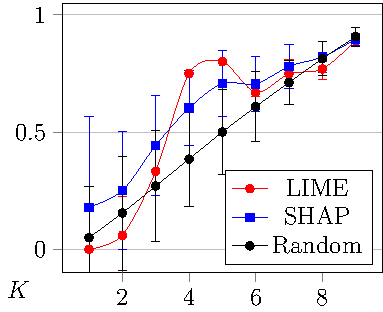
\includegraphics[width=\textwidth]{Figs/sec4_1-figure2.pdf}%
    %   \caption{Relevance}%The average and standard error of recall of SHAP and LIME when attempting to capture the top K most important features to $\mathcal{G}$ when explaining $\mathcal{M}$, for varied $K=1,2,3,...$ number of features.}
    %   \label{fig:avg_recall}
    %   \end{subfigure}
    %   \caption{Bar plot of directionality, violin plot of concordance, and line plot for relevance$_k$. For plot (c) Each point in the line plot represents a mean relevance for a given $k$. The error bars represent the standard error. The total number of features is 10.}
    %  \label{fig:beta_alignment}
    % \end{figure}  
  
  
\vspace{-3mm}  \subsection{Causes of Misalignment}
    \label{sec:causes_of_misalignment}\vspace{-3mm}
    We investigate factors in the pipeline that contribute to misalignment in terms of sign, relative importance, and relevance compared to the ground truth marginal effects, as aforementioned. Our aim is to provide both theoretical and empirical evidence for why post hoc explanations should not be used to make inferences about the actual input-output relationships underlying data. Our investigation will examine both stages of the explanation pipeline (the prediction stage and the explanation stage). % We first investigate SHAP and LIME in the explanation stage to show how their inherent model design contributes to misalignment. 
    We work under the assumptions that domain knowledge about the data generation process is unavailable. The experiments in this section involve first training an ML model $\mathcal{M}$ and then building an explainer model $\mathcal{E}$ to produce explanations. % training data to build a machine learning model and then and explanations of predictions of those MLPs on instances from the remaining 20\% of data reserved as a test set.
    


  \subsubsection{Explainers May Inherently Be Misaligned}
  \label{sec:theoretical_considerations}
  We first investigate how the explainers themselves contribute to misalignment by analyzing the equations for their explanations of linear models. To exclude other factors in the explanation pipeline, we consider an abstract scenario in which we explain $\mathcal{G}$ directly with SHAP and LIME. Thus, alignment is solely based on the explanation stage. We set $\mathcal{G}$ to be a linear function of $d$ i.i.d. normal features, i.e. $\mathcal{G}(\mathbf{x}) = \boldsymbol{\beta}^T \mathbf{x}$ where $\mathbf{x} \sim \mathcal{N}(\mathbf{0},\mathds{1}_d)$. SHAP and LIME explain the output of $\mathcal{G}$ at points $\boldsymbol{\xi}$, so the explicanda under consideration are $\boldsymbol{\beta}^T \boldsymbol{\xi}$ where $\boldsymbol{\xi}$ is a realization of $\mathbf{x}$. Below, we discuss how the underlying mathematical representations of SHAP and LIME explanations determine their inability to correctly identify $\boldsymbol{\beta}$. 


\vspace{-3mm} 
     \paragraph{$e_{\text{SHAP}}$ when Explaining a Linear Model}
       %SHAP does \emph{not} recover $\boldsymbol{\beta}$ and should not be relied upon for this purpose. 
       The importance of the $j^{th}$ feature of the $i^{th}$ data sample $\xi^{(i)}_j$ in a SHAP explanation is the Shapley value for feature $j$ in the prediction of sample $i$. The Shapley value reduces to the following expression when SHAP is used to explain a linear model according to \cite{StrumbeljErik2014Epma,lundberg17shap}: $e_\text{SHAP}(\mathbf{x}^{(i)}_j) = \beta_j (\xi^{(i)}_j - \bar{x}_j)$. 
       % \begin{equation}
       %  \label{eqn:shap_gt}
       %  e_\text{SHAP}(\mathbf{x}^{(i)}_j) = \beta_j (\xi^{(i)}_j - \bar{x}_j).
       % \end{equation}
    This formula highlights that SHAP explanations exhibit several undesirable properties that can limit their practical application. For instance, when $\boldsymbol{\xi}=\bar{\mathbf{x}}$, the SHAP values $e_\text{SHAP}$ reduce to 0, leading to all features being deemed unimportant. Moreover, SHAP values cannot be used to infer the signs of marginal effects because when $\xi^{(i)}_j - \bar{x}_j$ is negative, the signs of $e_{\text{SHAP}}(\xi^{(i)}_j)$ and $\beta_j$ are opposite. 
      %%Additionally, it is derived from Equation \ref{eqn:shap_gt} that the expected SHAP values average to zero, rendering them generally uninformative about the marginal effects. Some authors address this in their search for global feature importance by instead considering empirical averages of absolute SHAP values \cite{lenaers23rent,maeng23vr,guenther2023useful}. However, this obviously comes at the cost of losing information about the directionality of a feature's impact.
     %  To adjust for these undesirable properties of SHAP, we propose to normalize the SHAP values: $e_{\text{SHAP}}(\xi^{(i)}_j) / (x^{(i)}_j - \bar{x}_j)$. We refer to these as \emph{normalized SHAP values}. 
       
       %Although this is a straightforward adjustment one can make to in order to approximate the marginal effects using SHAP, we are not aware of it being used in prior literature. Our empirical evaluation of these normalized Shapley values, which includes recalculating directionality, concordance, and comparison with traditional SHAP results (illustrated in Figures \ref{fig:beta_alignment} and \ref{fig:shap_dividex_corr}), suggests significant improvements. Normalized SHAP values frequently exhibit correct sign alignment and generate feature rankings highly concordant with ground truth. Directionality for features related to credit score improved remarkably, as shown in Figure \ref{fig:shap_dividex_accs}. However, directionality for the features related to cosigner (married and cosigner) possession decreased somewhat. The improvement to feature rankings are evident from Figures \ref{fig:shap_dividex_spearmans} and \ref{fig:shap_dividex_recalls}; we can see that mean concordance rose from near 0 to about .6 and relevance was improved substantially for $k=2,3,4,5$. 
       
      
    %   Given the demonstrated effectiveness of the SHAP normalization scheme and our evidence that unmodified SHAP explanations are so inherently data-misaligned such that they are comparable to random explanations, \textbf{we will adopt this normalization approach for all subsequent experiments detailed in this paper}. This is vital as we explore the impacts of $\mathcal{M}$'s predictive performance and feature independence in subsequent sections (\ref{sec:role_of_predictive_power} and \ref{sec:role_of_correlation}). 
    %  \begin{figure}[ht!]
    %   \centering
    %   \begin{subfigure}[t]{.2\textwidth}
    %    \centering
    %    \captionsetup{justification=centering}
    %      \raisebox{.2cm}{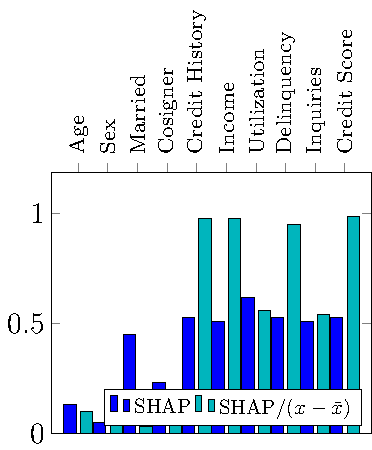
\includegraphics[width=\textwidth]{Figs/sec4_1-figure3.pdf}}%{Figures/lime_shap_Spearman_magnitude.png}

    %    \caption{Directionality}%Spearman rank correlations of feature importance magnitudes from SHAP and LIME against the true ranking from $\mathcal{G}$. }
    %    \label{fig:shap_dividex_accs}
    %   \end{subfigure}%
    %   \hspace{1cm}%\hfill
    %   \begin{subfigure}[t]{.2\textwidth}
    %    \centering
    %    \captionsetup{justification=centering}
    %    \raisebox{.05cm}{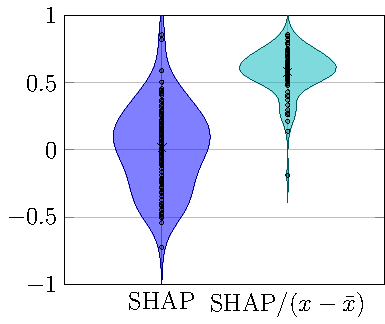
\includegraphics[width=\textwidth]{Figs/sec4_1-figure4.pdf}}%{Figures/lime_shap_Spearman_signed.png}
    %    \caption{Concordance}%Spearman rank correlations of signed feature importance from SHAP and LIME against the true ranking from $\mathcal{G}$.}
    %    \label{fig:shap_dividex_spearmans}
    %   \end{subfigure}
    %   \hspace{1cm}%\hfill
    %   \begin{subfigure}[t]{.2\textwidth}
    %    \centering
    %    \captionsetup{justification=centering}
    %   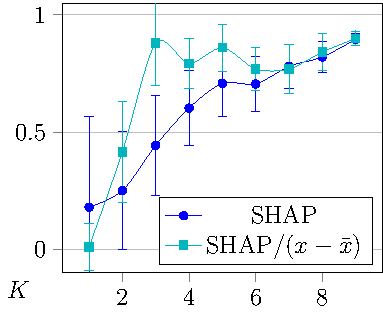
\includegraphics[width=\textwidth]{Figs/sec4_1-figure5.pdf}%
    %   \caption{Relevance}%The average and standard error of recall of SHAP and LIME when attempting to capture the top K most important features to $\mathcal{G}$ when explaining $\mathcal{M}$, for varied $K=1,2,3,...$ number of features.}
    %   \label{fig:shap_dividex_recalls}
    %   \end{subfigure}
    %   \caption{Comparison of SHAP explanations without and with SHAP value normalization}
    %  \label{fig:shap_dividex_corr}
    % \end{figure}  

    \vspace{-3mm}
    \paragraph{$e_{\text{LIME}}$ when Explaining a Linear Model}
      \label{sec:lime_linear_case}
       %In this section we we will show that there are conditions when the LIME coefficients have the property $e(x_j)\simeq \beta$ and use this fact to justify that $e(x_j)$ can be evaluated with respect to the ground truth $\boldsymbol{\beta}$. Those conditions are discussed in the next paragraph. 
       Local Interpretable Model-agnostic Explanations (LIME) works by sampling data points around a given instance, then using these samples to train a weighted linear model as a local surrogate model that approximates the predictions of the complex black box model in the vicinity of the instance. The linear model can be viewed as the solution to a kernel weighted regression with a sparsity penalty. The weights and the sparsity penalty, as well as the default behavior of numerical feature discretization, bias LIME away from recovering the linear model being explained \citep{han22which}.
       
       % To obtain interpretable and sparse explanations, LIME incorporates discretizes numeric features and includes a regularization component to promote sparsity in the local surrogate models it creates. This regularization helps in selecting a subset of features that are most influential for predictions near the instance being explained, thus ensuring that the explanations are both interpretable and concise. However, the above aspects of LIME's design may compromise its ability to accurately recover the true marginal effects coefficients. 
       
       % The use of discretized features in the regression model can eliminate critical information about the decision boundary of the model being explained. Additionally, LIME's reliance on ridge regression incorporates a sparsity penalty, which may lead to zeroing out coefficients for features where $\beta_j$ is indeed non-zero, distorting the picture one may obtain of the marginal effects. Moreover, employing weighted ridge regression introduces a weight matrix that further skews the estimation of marginal effects. This distortion can be observed in the closed-form solution of the weighted ridge regression, indicating potential limitations in LIME's ability to provide accurate estimates under certain conditions.

       Having identified the aforementioned properties of LIME's regression design as contributors to its lack of data-alignment, we derive Theorem \ref{thm:lime_thm}\footnote{Due to space limitations, the proof is available upon request.} below, which provides necessary conditions for LIME's data-alignment. It states that the expected coefficients of LIME without discretized features converge to $\boldsymbol{\beta}$ as the number of samples $n$ tends to infinity when explaining a linear model whose input features are i.i.d. normally distributed. It also gives a description of an ideal usage of LIME: explaining the prediction of linear function of numerical i.i.d normal features using an arbitrarily large sample of data around the input. This scenario cannot be realized in practice because we cannot guarantee the normality of input features, and it is of course not possible to create arbitrarily large data samples. As a consequence of the finiteness of the samples LIME creates, the weights and sparsity penalty matter in the weighted ridge regression, preventing recovery of $\boldsymbol{\beta}$.


      \begin{theorem}
        \label{thm:lime_thm}
        Suppose $f:\mathbb{R}^d\rightarrow \mathbb{R}$ that maps $\mathbf{x} \mapsto \boldsymbol{\beta}^T \mathbf{x}$, is explained at a sample $\boldsymbol{\xi}$ drawn from $\mathcal{N}(\mathbf{0}, \mathds{1}_d)$ with LIME. Let LIME use a generalized ridge regressor as a surrogate model with sparsity penalty parameter $\lambda=1$ and shrinkage target equal to the identity matrix $\mathds{1}_d$. Suppose further that LIME uses all features in the explanation, does not discretize them, samples i.i.d. data points $\mathbf{x}^{(1)},\ldots,\mathbf{x}^{(n)}$ from $ \mathcal{N}(\boldsymbol{\xi}, \mathds{1}_d)$, and weights those samples with the exponential kernel $\pi(\boldsymbol{\xi},\mathbf{x}) = exp(-\norm{\boldsymbol{\xi}-\mathbf{x}}_2^2/2\nu^2)$ using bandwidth $\nu>0$. Then, in the large $n$ limit, the coefficients of LIME converge to $\boldsymbol{\beta}$. That is, for each $\mathbf{x}^{(i)}$, $e_{\text{LIME}}(x^{(i)}_j) \rightarrow \boldsymbol{\beta}$
        as $n \rightarrow \infty$.
      \end{theorem}
       
       
       These settings make LIME's regression behave more like OLS than weighted ridge regression, such that the expectation of $e_{\text{LIME}}(\boldsymbol{\xi})$ over possible data samples is exactly $\boldsymbol{\beta}$. We do not allow LIME to use discretization in this section so that its values represent the importance of features instead of feature ranges. We demonstrate the advantage of the other settings in Section \ref{sec:mitigation_strategies}. 
 

  \subsubsection{Role of Predictive Power of $\mathcal{M}$}
    \label{sec:role_of_predictive_power}
      % The goal of the explanation pipeline is to unveil the underlying $\boldsymbol{\beta}$ within the unobservable structure $\mathcal{G}$. 
      Another factor in the pipeline that has a significant impact on  explanation alignment is the machine learning model $\mathcal{M}$ itself. 
      An explainer $\mathcal{E}$ is never directly applied to $\mathcal{G}$ because is $\mathcal{G}$ generally not directly observable. Instead, $\mathcal{M}$ is constructed based on data derived from $\mathcal{G}$ first, and it is this model to which the explainer $\mathcal{E}$ is applied. Consequently, it is reasonable to infer that the fidelity of $\mathcal{M}$ with respect to $\mathcal{G}$—that is, how accurately $\mathcal{M}$ reflects the true structure of $\mathcal{G}$—significantly influences the data-alignment of explanations. This fidelity is reflected by the predictive performance of $\mM$. 
      
      We test our intuition here by comparing SHAP and LIME explanations of three MLPs with different performance levels: test set ROC AUC of $0.60$, $0.90$ and $0.99$. %$\mathcal{M}_1$ with test ROC AUC $\simeq 0.60$, $\mathcal{M}_2$ with AUC $\simeq .93$, and $\mathcal{M}_3$ with AUC $\simeq 0.99$.
      %%When training $M_1$ and $M_3$, they start out as the same model (via random seed initialization) but are trained for sufficiently many epochs to achieve their corresponding AUCs of .6 and .93, respectively. Moreover, we follow Equation \ref{eqn:shap_gt} and normalize the SHAP values in this experiment, thereby bypassing SHAP's inherent data-misalignment and enabling us to show how increasing model AUC can aid the usage of SHAP. 
      %The results are shown in Figure \ref{fig:mlp_auc_increase} and demonstrate the positive relationship model performance has on data-alignment for both SHAP and LIME.
      The results of our comparison are displayed in Figure \ref{fig:mlp_auc_increase}, which shows that as the predictive performance of $\mM$ improves, the post hoc explanations are more aligned with the ground truth with respect to all three metrics. %Therefore, it is always recommended to build an ML model as accurate as possible in the prediction stage of the pipeline. 
      
      However, the near-perfect predictive performance of $\mM$ does not necessarily yield perfectly data-aligned explanations. As shown in the experiments, despite the third MLP achieving near-perfect performance via an AUC of $.99$, neither SHAP nor LIME were able to yield explanations perfectly aligned with the data. This is because perfect accuracy still does not guarantee that $\mM$ perfectly captures $\mG$. $\mathcal{M}$ represents a mapping from inputs to outputs. However, the training of $\mM$ only aims to obtain the correct outputs without controlling whether the mapping accurately reflects the true relationships underlying the data. In other words, it does not govern \emph{how} predictions are produced. Perfect accuracy only means that $\mM$ reaches the correct destination (i.e., the correct $Y$), but could likely take a different route to reach that destination. Thus, there is no guarantee of $\mathcal{M}$ being a perfect proxy for $\mG$, even if $\mM$ has perfect accuracy. 
      
      On the other hand, however, low accuracy is more strongly associated with low quality of $\mM$ in terms of capturing $\mG$, so it is generally recommended to try to optimize the predictive performance of $\mM$ in the explanation pipeline.

   

  %https://stats.stackexchange.com/questions/15011/generate-a-random-variable-with-a-defined-correlation-to-an-existing-variables
  \vspace{-3mm} 
  \subsubsection{Role of Feature Independence}
    \label{sec:role_of_correlation}\vspace{-3mm} 
% A machine learning model $\mathcal{M}$ is developed through training on a dataset $\mathcal{D}$, aiming to optimize predictive performance. $\mathcal{M}$ then represents a mapping from inputs to outputs. However, this outcome-based optimization ensures only the accuracy of the predictions without controlling whether the mapping accurately reflects the true relationships underlying the data. In other words, it does not govern \emph{how} predictions are produced. 
Machine learning reconstructs the mapping from the inputs to the outputs in a dataset, trying to reproduce the correct labels during training. However, an underlying problem with machine learning models is that they tend to overvalue features that provide information about multiple other features, as these are strong predictors of the target. 
% In real-world scenarios, features are typically interdependent. Thus, while the ideal model might rely predominantly on a specific set of features to determine the correct label, 
% $\mathcal{M}$ might infer using a different, albeit similar, set of features. Consequently, 
% $\mathcal{M}$ can arrive at the same predictions through an alternate mapping.
% Complicating this issue is the fact that, regardless of opinions on the significance of dependent variables, machine learning models tend to overvalue features that provide information about multiple other features, as these are strong predictors of the target. Post hoc explainers then interpret the importance of such features in various ways, further muddying the understanding of feature relevance within an ML model.
Therefore, the dependence of features can skew the perceived importance in a model, and this importance may be estimated by an explainer and subsequently used to draw incorrect conclusions about the data. % information about marginal effects. %it is crucial to investigate whether there is a discrepancy between the importance of interdependent features as assessed by a post hoc explainer and their significance as represented by their marginal effects. 

To demonstrate the impact of feature dependence, we generate a modified version of the dataset from Section \ref{sec:data_generation} with mutually independent features. In the original dataset, the credit score feature was a linear function of credit utilization, credit inquiries, delinquencies, and credit history. Possession of a cosigner was a function of marital status. In this revised dataset, the credit score is independent of all other features and the cosigner feature is now modeled as a Bernoulli-distributed random variable, independent of marital status. In this case, the marginal effects $\boldsymbol{\beta}$ of $\mathcal{G}$ match the coefficients in Equation \ref{eqn:gt}. %We normalize the SHAP values in an effort to show how feature independence can affect explanations obtained from SHAP, in spite of its inherent data-misalignment.

    Our experiment showed that by making credit score and cosigner independent, data-alignment increased overall and with respect to credit score and cosigner in particular. Indeed, Figure \ref{fig:lime_shap_colinear} shows that the directionality for those features increased for both SHAP and LIME. The figure also shows that mean concordance and mean relevance for almost all $k$ were larger for explanations of the model trained on the version of the dataset with independent features. 
   

\vspace{-3mm}  \subsection{Pervasiveness of Data-Misalignment}
    \label{sec:pervasive}\vspace{-3mm}
    We used one simulated dataset to demonstrate the mis-alignment of the SHAP and LIME explanations. To study how pervasive the issue is, % We show that data-misalignment is a general property of SHAP and LIME. In doing this, the implications of Section \ref{sec:causes_of_misalignment} are corroborated and the scope of their validity is widened. We do this by evaluating the data-alignment of 
    We evaluate the SHAP and LIME explanations using 100 simulated datasets. To do that, we randomly generate binary classification datasets with between 3 and 100 i.i.d normally distributed features and between 100 and 10000 rows.  The targets of the datasets are initially produced using randomly generated linear decision boundaries, but are then corrupted with varying amounts of noise. We generate a model for each dataset using the Python AutoML package auto-sklearn. Their test set accuracies are between $.82$ and $.99$. It is important to note that as the features are normally distributed and mutually independent, this scenario is practically ideal.  
    %%We do not allow the AutoML to perform feature pre-processing. We set the AutoML to search among the following model types: MLP, XGBoost, Decision Tree, ExtraTrees, Random Forest, and \textcolor{red}{\ldots}. The models are evaluated using 5-fold cross validation with respect to test set accuracy. We run the AutoML in a parellelized fashion with 16 cores and allow a maximum of 10 minutes to produce a model for each dataset. 

    Since the number of features differs across the datasets, we report the results for our three metrics in the following fashion, conditioned on the number of features $d$. For each dataset with $d$ features, we compute the feature-wise mean directionality over $m=100$ test set instances and report the average over the datasets. Similarly, we report the mean and standard deviation of concordance, and mean relevance for $k=3$. 




    
    Our experimental results imply that SHAP and LIME explanations are generally not informative about marginal effects for datasets with more than thirty features. Indeed, Figure \ref{fig:lime_shap_vary_d} shows that, generally when $d$ exceeds $30$, mean directionality for SHAP and LIME is actually under $.5$, worse than random guessing. This is an alarming sign because the two most popular post hoc explainers can not even get the correct qualitative estimation of the true marginal effect - even the sign is wrong! In addition, both the mean concordance and mean relevance for $k=3$ are near $0$. It should be noted that the more features there are, the more challenging it is for the two explainers to correctly identify the contributions of each feature, as there exist more possible mappings from the input to the output that could be different from that of $\mG$ and there is no control over which one $\mM$ uses.

\vspace{-3mm}  \subsection{Discussion}\vspace{-3mm}
      Since researchers cannot directly access the ground truth model $\mathcal{G}$ and can only interact with an intermediary machine learning model $\mathcal{M}$, the explanation process is bifurcated into two distinct stages: the prediction stage and the explanation stage. 
      We find that challenges arise in both stages, necessitating additional assumptions about the data $\mathcal{D}$, $\mathcal{M}$, and the explanation tool $\mathcal{E}$. Crucially, $\mathcal{E}$ must possess the ability to accurately capture information regarding the marginal effects. The discussion in Section \ref{sec:theoretical_considerations} describes theoretically why it is challenging for SHAP and LIME to draw even qualitative information (e.g. the sign) of the true marginal effect. In addition, the predictive performance of $\mathcal{M}$, the independence of features, and the number of features also have a significant impact on the resulting explanations. %Insights from Section \ref{sec:causes_of_misalignment} indicate that $\mathcal{M}$'s ability to achieve high predictive accuracy, especially when trained on data with mutually independent features, significantly facilitates the extraction of the marginal effects. 
      \textbf{SHAP and LIME being data-misaligned appears to be a general phenomenon}, which worsens with \textit{low predictive performance of the machine learning model, dependence of features, and the large number of features}. 



    
\vspace{-3mm}\section{The Mitigation Strategies}
  \label{sec:mitigation_strategies}\vspace{-3mm}
  So far in this paper, we have established that there exists serious flaws in using post hoc explanations to infer the ground truth feature insights from data. In this section, we propose mitigations to see if we can improve the quality of the explanations. We will test mitigation strategies using real loan application data from the Federal Reserve Bank of Boston \citep{hunter1996cultural} and compare the findings with those reported in an econometric publication \citep{bane2006econometric}.
    
\vspace{-3mm}   \subsection{Mitigation Strategies}
    \vspace{-3mm} 
    Several mitigation strategies follow, beginning with strategies specific to SHAP or LIME, and ending with generally applicable ones. Our strategies are meant to be sufficiently simple to understand and use such that they form a platform for further exploration and experimentation. 
    
    \noindent\textbf{Normalizing SHAP Values}
        It follows directly from the theory underlying SHAP that SHAP values are not marginal effects and so it is therefore worthwhile to seek practical ways to modify our usage of SHAP. As SHAP returns $e_{\text{SHAP}}(\mathbf{x}^{(i)})=\boldsymbol{\beta}^T(\mathbf{x}^{(i)} - \bar{\mathbf{x}})$ instead of $\boldsymbol{\beta}$ when explaining $\boldsymbol{\beta}^T \mathbf{x}^{(i)}$,  we propose to normalize the SHAP values using $e_{\text{SHAP}}(\xi^{(i)}_j) / (x^{(i)}_j - \bar{x}_j)$ where $\bar{x}_j$ is the empirical mean of feature $j$ from the training data because this expression should be approximately $\beta_j$. We refer to these as \emph{normalized SHAP values}.  %we proposed in Section \ref{sec:theoretical_considerations} to instead take the importance of feature $j$ to be $e_{\text{SHAP}}(x^{(i)}_j) / (x^{(i)}_j - \bar{x}_j)$ where $\bar{x}_j$ is the empirical mean of feature $j$ from the training data because this expression should be approximately $\beta_j$. %Our experiments confirmed the advantage of this technique.
        
        % Figure \ref{fig:shap_dividex_corr} showed that unmodified SHAP explanations perform about as well as random ones with respect to our three metrics while the normalized SHAP explanations performed quite well with respect to our three metrics. In addition, the normalized SHAP explanations were more consistent across individuals (recall that Figure \ref{fig:shap_dividex_spearmans} showed that the concordance distribution for normalized SHAP explanations had a significantly smaller region of support which, importantly, was centered at a larger value than the mean concordance of the unmodified SHAP explanations). 
        %%Since these results were produced using the version of our dataset with correlated features, we additionally provide a comparison of SHAP without and with normalization when the input features are independent in Appendix Section \ref{sec:shap_norm_indep}.



    
    \noindent\textbf{Setting hyper-parameters of Post Hoc Explainers} 
      \label{sec:lime_params}
      %\textcolor{red}{Our theorem in section XX shows that ..... Motivated by the theorem, we propose ...}
      Theorem \ref{thm:lime_thm} in Section \ref{sec:theoretical_considerations} shows that in an ideal use-case for LIME wherein we assume that LIME is not using feature discretization, the expected LIME coefficients tend to the marginal effect values $\boldsymbol{\beta}$ as the number of samples $n$ synthesized for its underlying regression tends to infinity. Motivated by the theorem and the impossibility of creating arbitrarily large data samples in practice, we propose that $n$, as well as LIME's kernel bandwidth $\nu$, need to be large in order for $e_{\text{LIME}}(x_j)$ to be close to $\boldsymbol{\beta}$. We suggest, e.g., setting $n=\nu=10000$ rather than the default settings of $n=\sqrt{.75d}$ and $\nu=1000$. These settings make LIME's regression behave more like OLS instead of weighted ridge regression.
      
     

      \noindent\textbf{Averaging Explanations of One Model by Different Explainers}
      \label{sec:averaging_one_explainer}
      %Although the inconsistency of the explanations referenced in the related work (Section \ref{sec:related_work}) is unfortunate because it makes individual explanations seem less plausible, 
      The issue of explanation inconsistency, which happens when many distinct and possibly conflicting explanations of the same prediction can be obtained, is a well known problem in the XAI literature \cite{alvarez18robustness}. 
      We propose that it can actually be leveraged into an advantage. Each explanation likely has at least a modicum of truth, and so an aggregation strategy for explanations may increase the signal-to-noise ratio. We propose here one simple realization of this general idea. Given one ML model $\mathcal{M}$ and instance $\mathbf{x}$, we leverage the abundance of possible LIME explanations of $\mathcal{M}(\mathbf{x})$ by averaging the feature importance values given by a set of LIME explainers with different random seeds. %%We have found that there is a tendency for an explanation constructed using the average feature importance values over a set of LIME explainers with different hyperparameters to be superior to single explanations from LIME with its default settings. %%We do not test this strategy with SHAP since its explanations at the individual level are deterministic. 

   \noindent\textbf{Optimizing the Tradeoff between Complexity and Predictive Power}
      \label{sec:decreasing_complexity}
      In view of the facts that 1) given some dataset, many models $\mathcal{M}$ exist with approximately the same generalization error \citep{semenova22rashomon} and 2) the complexity (number of parameters) of a model is a basic factor that distinguishes it, it makes sense to analyze what role the complexity of $\mathcal{M}$ plays on data-alignment. We have identified that models which are needlessly over-parameterized in that the same (or better) performance can be obtained by a simpler model may be less faithful to $\mathcal{G}$ due to having unnecessary variation in their decision boundaries.\footnote{This is similar to the phenomenon in least squares polynomial regression where $r^2$ increases with the degree of the regressors regardless of how simple the mapping underlying the dataset is}.
      Since we established in \ref{sec:role_of_predictive_power} an association between the predictive performance of $\mathcal{M}$ and the faithfulness of explanations of $\mathcal{M}$ with respect to $\mathcal{G}$, we propose that researchers should ensure that $\mathcal{M}$ has both good predictive performance and minimal complexity.
      %%The labels predicted by $\mathcal{M}$ (after thresholding its output probabilities) agreeing with those in the test set is an incomplete representation of faithfulness to $\mathcal{G}$; even if $\mathcal{M}$ had 100\% training and testing accuracy on data with no measurement error this does not mean $\mathcal{M}=\mathcal{G}$. Thus, it is worth making an effort not to over-parameterize $\mathcal{M}$. To carry out this strategy, one can iteratively train and evaluate models of successively lower complexity and stop the procedure once the reduction of complexity leads to a substantial reduction in predictive performance. 
      
      %%To investigate this tradeoff as it pertains to data-alignment, we compare SHAP and LIME explanations of two MLPs (perceptrons, actually) of differing complexity but essentially the same predictive performance. The first MLP, $\mathcal{M}_1$, has 100 nodes in its hidden layer (the default in sklearn) and a test set AUC of about $.99$. The second, simpler MLP $\mathcal{M}_2$, has only two nodes in its hidden layer and yet also has a test set AUC of about $.98$. Figure \ref{fig:decreasing_complexity} visualizes our comparison of explanations of $\mathcal{M}_1$ and $\mathcal{M}_2$. %%Additional results and further motivation for this strategy can be found in Appendix Section \ref{sec:appendix_inconsistency}.

      %%We found that with the exception of relevance for SHAP, all three metrics were improved for both explainers. However, as shown by Figure \ref{fig:decreasing_complexity}, the improvements were marginal for the most part.
      %%For SHAP, we reject the null hypothesis of equal sign accuracies only for age with a p-value of $2.76e-9$ and credit history with a p-value of $0.04$. It is evident from Figure \ref{subfig:decreasing_complexity_shap_spearmans} that concordance did not rise significantly; we failed to reject the null hypothesis of equal concordances with a p-value of $.16$. Although relevance worsened for $k=8$ when explaining $\mathcal{M}_2$, the small improvements for $k=1,2,4,5,6,7$ were significant all with $p<.001$ except for $k=4$, which had $p=4.73e-2$.% $6.21e-3$, $9.83e-4$, $4.73e-2$, $7.85e-5$, $9.73e-6$, and $8.17e-17$.
      %%For LIME, we could only conclude that the directionality of ``married" improved by rejecting the null hypothesis of equal directionality with a p-value of $0.015$. However, the improvement to concordance was significant as its test had a p-value of $4.90e-5$. As for relevance, the results for $k=1$ were identical and the null hypothesis of equal relevance was rejected in favor of improvement for $k=2,6$ with p-values of $0.02$ and $0.01$. 
      
      %%A reason that the explanations of the simple model $\mathcal{M}_2$ were better is that even though $\mathcal{M}_1$ may have similar behavior in how they generate training and test set labels, the additional expressive power of $\mathcal{M}_1$ allows the local behavior of its decision boundary to be more erratic. Given that SHAP and LIME are local function approximators, incorrect local behavior of $\mathcal{M}_1$ imposes a limitation on how data-aligned SHAP and LIME can be when explaining $\mathcal{M}_1$. 

   %simple models used here
    %\subsubsection{Tuning $\mathcal{M}$ with Minimal Complexity}
    %  \label{sec:m_fidelity}


      %We then demonstrated in Section \ref{sec:role_of_causal}, keeping the predictive performance of $\mathcal{M}$ approximately constant, that (LIME) explanations of a model $\mathcal{M}$ were better equipped to recover $\boldsymbol{\beta}$ when $\mathcal{M}$ was trained on data without correlation or confounding. Whenever possible, it is therefore worthwhile to pre-process data in a way that accounts for correlated and confounded features. %We will show in Appendix Section \ref{sec:backdoor_adjustment} a way to do this that requires knowledge of the true structural causal model underlying the dataset. 

    %\subsubsection{Near Perfect Test Set Accuracy of Model Trained on Ideal Dataset}
      %\label{sec:optimal_conditions}
      %This mitigation strategy relies on the intuition that post hoc explanations should have the best results when the conditions for their use are practically ideal in the senses that 1) $\mathcal{M}$ has very high test set AUC and 2) the data set satisfies the causal inference conditions. To satisfy the two aforementioned conditions, we again use the low-dimensional dataset with no causal inference violations from Section \ref{sec:causes_of_misalignment} but train $\mathcal{M}$ so that attains 99\% test set accuracy and an AUC of .98.
      
      %. Figure \ref{fig:lime_shap_g} shows that, when explaining $\mathcal{M}$, LIME is able to extract the true feature ranking and gets close with high consistency. SHAP usually does not recover the true feature Spearman Rank Correlations and additionally has more variance in the ranking distribution. %When explaining $\mathcal{G^*}$ itself, LIME seems to be able to perfectly recover the true ranking order almost always. When explaining $P_1$, SHAP can actually recover the true feature Spearman Rank correlations, but with less consistency than LIME does. 
    
      %We repeat the experiments of Section \ref{sec:evaluating_faithfulness} once more, but this time explain the aforementioned highly accurate model. Our results appear in Figures \ref{fig:perfect_data_model}. The main difference between we observed after raising the AUC of $\mathcal{M}$ from .95 to .99 occured with respect to the recall metric. Most notably, we can see from Figure \ref{fig:perfect_data_model_recalls} that LIME's average $\text{relevance}_k$ was equal to 1 for $k=1,2$ and closer to $1$ for $k=3,4$ than in Figure \ref{fig:avg_recall}. SHAP's $\text{relevance}_k$ also improved both in terms of mean and variance over the 100 applicants. However, there was not a signicant difference in the sign accuracy and rank correlation metrics.
      
      %Moreover, SHAP and LIME both still admit the possibility of misalignment in this scenario, despite the conditions for their use being in some sense ideal. For example Figure \ref{fig:perfect_data_model_acc} shows that SHAP and LIME could still only correctly identify how age impacts loan application likelihood for about half of the applicants.% in 
  
\vspace{-3mm}    \paragraph{Averaging Explanations of Different Models}
      The rate at which new machine learning models and methods appear has exploded, making it increasingly difficult for researchers to choose what model to use and ultimately explain. Coupled with the fact that each of them has hyperparameters to tune, model selection is to a machine learning researcher as was finding a route to the Spice Islands to Magellan. A straightforward way to address concerns about what black box to explain is to train many models and construct an average explanation over those models. In this way, diverse information from the hypothesis space under consideration is included in the final (averaged) explanation.%Often, but depending on the data set, many different models can be constructed that have nearly the same predictive performance \citep{semenova22rashomon}. Each nevertheless has a distinct decision boundary and captures different correlations in the data, and so post hoc explanations of those models can still differ.
      
      
      %%With this in mind, we repeat the experiments of Section \ref{sec:evaluating_faithfulness} twice, once with explanations of a single model and again with the modification that concordance is calculated between the ground truth and a feature ranking constructed by averaging feature importance values over SHAP and LIME explanations of 100 unique MLPs with ROC AUC at least $.9$. The results of our Wilcoxon tests for improvement of data-alignment were quite different between SHAP and LIME.
      % PUT THESE DETAILS IN APPENDIX
      %Each MLP is trained with 5 hidden layers and for 10 iterations as before, but each MLP initializes its training with a different random seed. We control for the inconsistency of the explainers by using default hyperparameters and keeping the random seed of the explainers the same. 
       
      %%The results of our Wilcoxon tests for improvement of data-alignment were quite different between SHAP and LIME. These differences are visualized in Figure \ref{fig:mlp_increase}. Directionality, concordance, and relevance were all significantly improved for LIME. We rejected the null hypothesis of equal sign accuracies in favor of improvement for ``cosigner", ``married", and ``sex" with respective p-values of $0.04$, $4.56e-4$, and $2.87e-7$. We rejected the null hypothesis of equal concordances in favor of improvement as the p-value was $4.21e-11$. In contrast, there was no significant change to sign accuracy for any feature (all p-values were at least $0.15$) and no significant change to concordance, as we failed to reject the null hypothesis of equal concordances with a p-value of $0.25$. Figures \ref{subfig:mlp_avg_lime_sign_accs} and \ref{subfig:mlp_avg_lime_recalls} together show that LIME was had better estimates of the $\boldsymbol{\beta}$ coefficients for ``age", ``cosigner", married, and sex. In contrast, for SHAP, it is difficult to see any difference in directionality and concordance in Figure \ref{subfig:mlp_avg_shap_sign_accs} and Figure \ref{subfig:mlp_avg_shap_recalls}. %Our results are shown in Figure \ref{fig:mlp_increase}.
      
      %Figure \ref{subfig:mlp_avg_lime_spearmans} shows that LIME's averaged explanations had a slightly larger mean and slightly lower range while Figure \ref{subfig:mlp_avg_lime_spearmans} shows that concordance was almost unchanged for SHAP. Figures \ref{subfig:mlp_avg_lime_sign_accs} and for LIME and \ref{subfig:mlp_avg_shap_sign_accs} and \ref{subfig:mlp_avg_shap_recalls} show that, with a few exceptions, the averaged explanations were at least as good as the explanations of a single model at identifying feature importance signs and the top-$k$ features. 
      
      %However, the strategy does not seem to be particularly beneficial for finding the top-$k$ features; the curves plotting the recall for SHAP and LIME in Figures \ref{subfig:mlp_avg_lime_recalls} and \ref{subfig:mlp_avg_shap_recalls} are nearly identical for the averaged and single explanation.%Figure \ref{fig:mlp_avg_recalls} also shows that the curves representing the relationships between $K$ and recall for $n=100$ bound the other curves from above. Therefore, this strategy appears to be effective in reducing both misalignment and inconsistency.

      %%This strategy can be seen as a simplified version of \citep{donnelly2023rashomon}. Instead of leveraging explanations of good models trained on one dataset, they leverage explanations of optimal decision trees or GAMs trained on bootstraps of one dataset. At the time of writing, their method is not valid for more complex models like neural networks. It also produces statistics for feature importance instead of singular feature importance values. 
  

    % \begin{figure}[t!]
    %   \centering
    %   \subfloat[SHAP Directionality]{%
    %     \raisebox{.2cm}{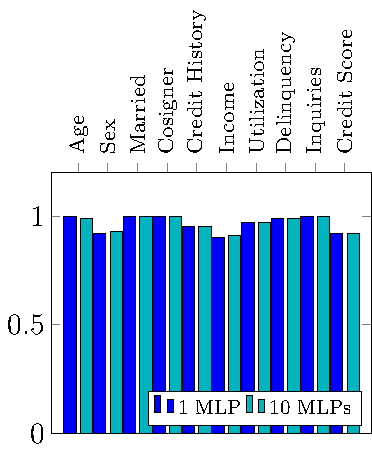
\includegraphics[width=.2\textwidth]{Figs/sec5_2_simple_mlp_avg-figure1.pdf}}%
    %     \label{subfig:mlp_avg_shap_sign_accs}%
    %   }\hspace{1cm}
    %   \subfloat[SHAP Concordance]{%
    %     \raisebox{.05cm}{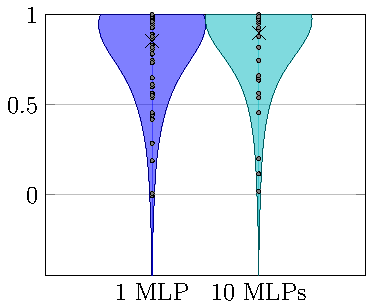
\includegraphics[width=.2\textwidth]{Figs/sec5_2_simple_mlp_avg-figure3.pdf}}%
    %     \label{subfig:mlp_avg_shap_spearmans}%
    %   }\hspace{1cm}
    %   \subfloat[SHAP Relevance]{%
    %     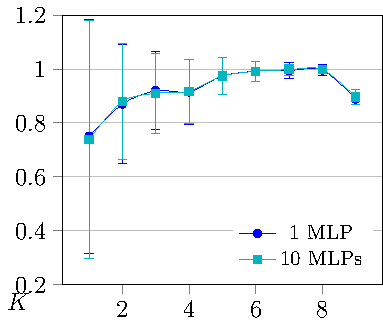
\includegraphics[width=.2\textwidth]{Figs/sec5_2_simple_mlp_avg-figure5.pdf}%
    %     \label{subfig:mlp_avg_shap_recalls}%
    %   }\\
    %   \subfloat[LIME Directionality]{%
    %     \raisebox{.2cm}{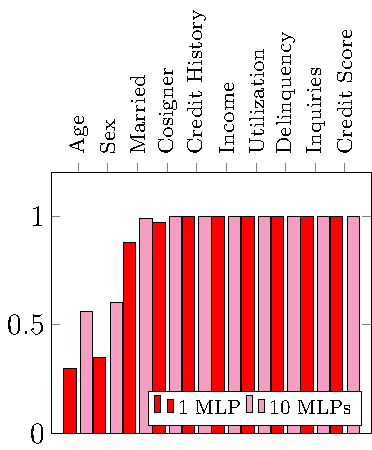
\includegraphics[width=.2\textwidth]{Figs/sec5_2_simple_mlp_avg-figure0.pdf}}%
    %     \label{subfig:mlp_avg_lime_sign_accs}%
    %   }\hspace{1cm}
    %   \subfloat[LIME Concordance]{%
    %     \raisebox{.05cm}{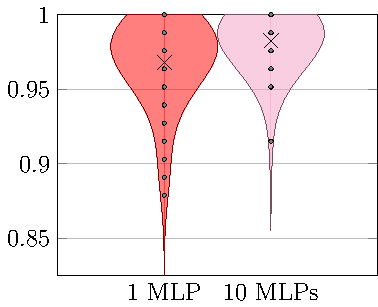
\includegraphics[width=.2\textwidth]{Figs/sec5_2_simple_mlp_avg-figure2.pdf}}%
    %     \label{subfig:mlp_avg_lime_spearmans}%
    %   }\hspace{1cm}
    %   \subfloat[LIME Relevance]{%
    %     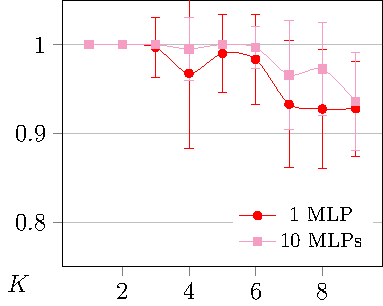
\includegraphics[width=.2\textwidth]{Figs/sec5_2_simple_mlp_avg-figure4.pdf}%
    %     \label{subfig:mlp_avg_lime_recalls}%
    %   }\\
    %   \caption{Comparisons of results for our three metrics for SHAP (top row) and LIME (bottom row) explanations of 1 MLP versus explanations constructed by averaging the feature importance values of 10 MLPs.}
    %   \label{fig:mlp_increase}
    % \end{figure}
    

  
  
  % \subsection{Summary and Discussion of Mitigation Strategies}
  %     \label{sec:summary_and_strategies}
  %     The main results of our mitigation experiments are that when using SHAP the Shapley values should be normalized, and when using LIME, it may be worthwhile to aggregate the explanations of many LIMEs and individual LIME explainers should have large $\nu$ and $n$. Secondarily, it may be worthwhile to seek black boxes that optimize the trade-off between complexity and predictive power and to average explanations over ensembles of explainers and/or models. 
  %     %It makes less sense to combine explanations of a single model than explanations of multiple models because of the idea that ``all models are wrong". 
      
  %     Finding common (valid) patterns within multiple black boxes is possible by aggregating explanations of those models whereas aggregations of explanations of a single black box can at best reveal the single, imperfect, pattern identified by that black box. Ignoring bias and error in the dataset, each explanation has two layers of approximation error with respect to the ground truth whereas each black box has only its own approximation error and captures different patterns in the training data. Thus, researchers may find averaging feature importance values obtained by many models both a useful and intuitive strategy\citep{dong2020variable,donnelly2023rashomon}. %With the configuration of data and model we used, the local error rates of both SHAP and LIME were skewed to the right, implying that the mean local fidelity over samples of SHAP and LIME models can decrease as the sample size increases. However, it is difficult to validate this claim because the local fidelity of SHAP and LIME is not an especially good measure of how faithful their explanations are to $\mathcal{G}$. That averaging SHAP and LIME together did not yield a consistent and substantial advantage is likely due to the simplicity of the technique. For this reason, we suggest that more research be done on this topic. 
      
  %     Summing up, researchers who would like to investigate the importance and impact of features in a data generating process may find exploring the following general strategy useful. First, the choice of explainer(s) used for the strategy should be guided by user preference for the types of feature importance outlined in Section \ref{sec:theoretical_considerations}. For example, LIME should be preferred to SHAP if $\boldsymbol{\beta}$ is preferred to $\boldsymbol{\beta}(\boldsymbol{\xi}-\bar{\mathbf{x}})$ as the ground truth feature importance representation. %construct average explanations over a collection of good LIME explanations of good models. If situational importance is more suitable than theoretical importance for the application, researchers should instead average over SHAP explanations of good models. 
  %     Next, when starting the prediction stage, the dataset should be pre-processed to remove highly correlated features\footnote{If possible, adjustments can be made to account for confounding. Tools like E-values\citep{gaster2023quantifying} and Pearl's backdoor criterion can be used for this purpose.}% The causal graph can be estimated using Bayesian Networks if sufficient domain knowledge is available.}
  %     Having pre-processed the data, researchers are encouraged to train $B\geq 1$ black box models with simple enough decision boundary/separating surface to not lose too much predictive performance compared to more complex models. \footnote{Ideally, Rashomon sets of models would be constructed and the simplest models in them would be collected. However, at the time of writing, this is only possible for decision trees and GAMs.} To construct an explanation for the predicted outcome of an instance, the results of multiple explainers can be aggregated by, e.g., averaging the feature importance values over the component explainers. Doing this for each of the $B$ models, $B\cdot E$ explanations in total are used to produce a final explanation for an instance.
      
  %     % \section{Testing the Recommended Pipeline}
  %     %   We will demonstrate the efficacy of our recommended pipeline by benchmarking it against a baseline pipeline on five new simulated datasets. The five datasets are have the following ground truths, which have increasing complexity. $\mathcal{G}_1$ is linear, but includes nonlinear transformations of $x$. $\mathcal{G}_2$ includes nonlinear transformations of the $x_i$ as well as an interaction term. $\mathcal{G}_3$ includes features which are correlated through another set of observed features. $\mathcal{G}_4$ has unobserved confounding. $\mathcal{G}_5$ additionally has an interaction term. 
      
  %     %   \begin{enumerate}
  %     %     \item $\mathcal{G}_1(x) = \mathds{1}[\sum_{i=1}^{10} \lambda_i log(x_i) > c_1]$ where $\lambda_i \in (0,1)$ and $x_i \sim \mathcal{U}(1,10)$ $\forall i$
  %     %     \item $\mathcal{G}_2(x) = \mathds{1}[\mathbf{\Sigma}(x_1x_2 + cos(x_2) + min(x_3,0) + exp(x_4/4) + x_5^2/2) > .5]$ and $x_i \sim \mathcal{U}(-1,1)$
  %     %     \item $\mathcal{G}_3(x) = \mathds{1}[\mathbf{\Sigma}(x_1 + 2x_2 + x_3/3 + 2x_4/3 + x_5)>c_4]$ where $x_1,x_2,x_3 \sim \mathcal{N}(0,1)$, and $x_4 = 2 + z_1$, $x_5 = 2 + 3 z_3$ where $z_3 = .8 z_1 + \sqrt{1-.8^2}z_2$ and $z_1\sim \mathcal{N}(1,1)$ and $z_2 \sim \mathcal{N}(2,9)$ with $z_1,z_2$ in the training data
  %     %     \item $\mathcal{G}_4(x)$ the same as $f_4(x)$ but without $z_1,z_2$ in the training data
  %     %     \item $\mathcal{G}_5(x) = \mathds{1}[\mathbf{\Sigma}(2x_1x_2 + \frac{1}{sin(x_3)} + 2x_4/3 + x_5)>c_5]$ where $x_1,x_2,x_3 \sim \mathcal{N}(0,1)$, and $x_4 = 2 + z_1$, $x_5 = 2 + 3 z_3$ where $z_3 = .8 z_1 + \sqrt{1-.8^2}z_2$ and $z_1\sim \mathcal{N}(1,3)$ and $z_2 \sim \mathcal{N}(.5,4)$ without $z_1,z_2$ in the training data. \textcolor{red}{Fenglu should pick $c_5$ such that the target is highly imbalanced.}
  %     %   \end{enumerate}
        
        
  %     %   Our baseline pipeline will be represented by a default LIME explanation of an MLP with a ROC AUC of about $.8$. To represent our recommended pipeline, we construct an average explanation for each applicant using the explanations of 10 MLPs with AUC $\geq .9$ by 10 LIME explainers that correctly classify the applicants' loan decisions. We attempt to find the minimum complexity that allowed the MLPs to attain AUC values that exceeded $.9$ to avoid needless model complexity and overfitting. 





%% \subsection{Case Study: Replicating Econometric Findings}
%   \label{sec:case_study}
%   To validate our efficacy of our mitigation strategies and illustrate how they could be employed in practice, we will compare how well two combined strategies reproduce insights from an econometric paper on the approval of home loan applications \citep{bane2006econometric} against two baselines. The home loan data set is publicly available and originates from a study by the Federal Reserve Bank of Boston \citep{hunter1996cultural}. We take the ground truth $\boldsymbol{\beta}$ underlying this data set to be the coefficients of the logistic regression model obtained in the analysis of \cite{bane2006econometric}. This is justifiable because econometric modeling is equipped to capture $\boldsymbol{\beta}$. The linear ground truth model derived from their logistic regression model appears in Equation \ref{eqn:econ_gt}. The meanings and ranges of each feature appear in Appendix Table \ref{tab:case_study_features}. %We will use the logistic regression coefficients to evaluate SHAP and LIME explanations in the same manner as has been done throughout this paper. We suppose that the logistic regression coefficients have the correct signs and magnitudes relative to each other, not that the logistic regression itself is the true causal model underlying home loan approvals in Boston. 

%   Our two combined strategies are versions of the general strategy outlined in Section \ref{sec:summary_and_strategies} tailored to SHAP and LIME. We will perform the following comparison to evaluate them. First, we split the data set into 80\% training data and 20\% testing data. Then we train 10 MLPs with test set AUC that are all near $.92$. The LIME variant of the strategy uses all $B=10$ MLPs and $E=10$ LIME explainers for each MLP. Each LIME explainer has $\nu=n=10000$. Because SHAP is (essentially) deterministic and the MLP averaging strategy did not significantly increase directionality and concordance for SHAP, we use $B=E=1$ and normalize the Shapley values. Baseline explanations come from explanations of one MLP with accuracy $.86$, ROC AUC $.93$ with individual SHAP and LIME explainers both using default settings. 
  
%   %\begin{tcolorbox}[title = Econometric Ground Truth Model $\mathcal{G}$]
%   \begin{equation}
%   \label{eqn:econ_gt}
%   \begin{split}
%     \mathcal{G}(X) =.8 + 3.5\cdot \text{good credit} + 4.7\cdot \text{purchaser type} -4.4 \cdot \text{PMI approved} - .4 \cdot \text{multi family} \\ -2.5 \cdot \text{unver} + .9 \cdot \text{fixed rate} - 1.4 \cdot \text{bankruptcy} - .9 \cdot \text{value rate} - .03 \cdot \text{debt rate} \\- .7 \cdot \text{old} + .8 \cdot \text{married} - .8 \cdot \text{gift}
%   \end{split}
%   \end{equation}
%   %\end{tcolorbox}
%   %\subsection{Baseline Performance}
%   %Figure \ref{fig:econ_cmp} compares the explanation quality for 100 applicants from the baseline pipeline and recommended pipeline. %In the Appendix, we show also compare results for importance sign accuracy, Spearman rank correlation, and recall.

%   Both the SHAP and LIME variants of our general strategy generally had results which improved upon the baseline in at least one respect. Indeed, our strategy applied to LIME significantly improved concordance overall, significantly improved directionality for ``fixadj" and ``old", significantly improved relevance for the top 2 and 3 features. It had significantly worse directionality only for ``vr" and ``obrat", and significantly worse relevance for features not in the top-4. Our strategy applied to SHAP significantly improved directionality for all features except ``fixadj" and ``gift", significantly improved concordance, and significantly improved relevance for all $k\neq 1,11$. 
  
%   %Figure \ref{fig:econ_cmp} visualizes the results. The directionality values from our recommended strategy with SHAP and LIME were at least as good as those from the baseline for all features except ``pubrec" (bankruptcy filed) for LIME and ``vr" (value rate) for SHAP (see Figures \ref{subfig:econ_lime_sign_accs} and \ref{subfig:econ_shap_sign_accs}). The concordance plots for both SHAP and LIME in Figures \ref{subfig:econ_shap_spearmans} and \ref{subfig:econ_lime_spearmans} show that the recommended pipeline rankings were generally more faithful than the most faithful explanations from the equivalent baseline. Finally, it can be seen from Figures \ref{subfig:econ_lime_recalls} and \ref{subfig:econ_shap_recalls} that the recommended strategies using SHAP and LIME both have substantially higher relevance for all $k\neq 1,\ 10,\ 11$.
   
% % \begin{figure}[!h]
% % \centering
% %   \begin{subfigure}[t]{0.2\textwidth}
% %   \centering
% %   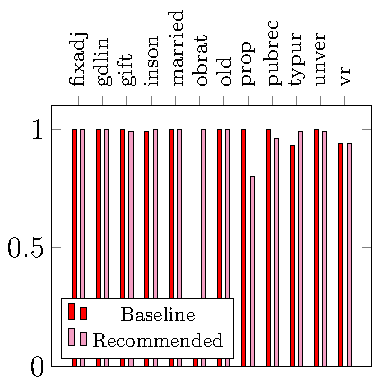
\includegraphics[width=\textwidth]{Figs/econ_cmp-figure0.pdf}
% %   \caption{Directionality} \label{fig:econ_cmp_sign_accs}
% % \end{subfigure}\hspace{1cm}
% % \begin{subfigure}[t]{0.2\textwidth}
% %   \centering
% %   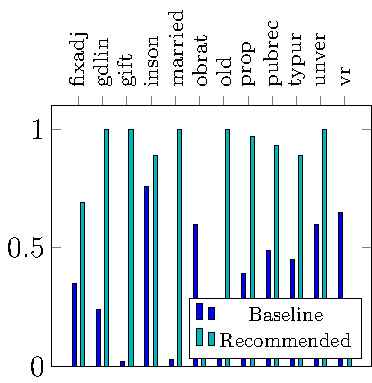
\includegraphics[width=\textwidth]{Figs/econ_cmp-figure1.pdf}
% %   \caption{Relevance} \label{fig:econ_cmp_spearmans}
% % \end{subfigure}\hspace{1cm}
% % \begin{subfigure}[t]{0.2\textwidth}
% %   \centering
% %   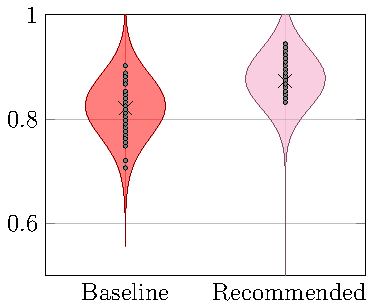
\includegraphics[width=\textwidth]{Figs/econ_cmp-figure2.pdf}
% %   \caption{Recall}
% %   \label{fig:econ_cmp_recalls}
% % \end{subfigure}
% % \caption{Improvements due to use of recommended pipeline instead of one without any of our mitigation strategies}\label{fig:econ_cmp}
% % \end{figure}


%     \begin{figure}[t!]
%       \subfloat[SHAP Directionality]{%
%         \raisebox{.2cm}{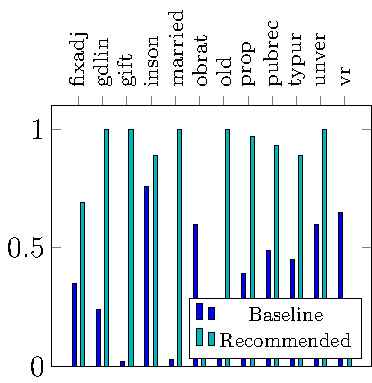
\includegraphics[width=.2\textwidth]{Figs/econ_cmp-figure1.pdf}}%
%         \label{subfig:econ_shap_sign_accs}%
%       }\hspace{1cm}
%       \subfloat[SHAP Concordance]{%
%         \raisebox{.05cm}{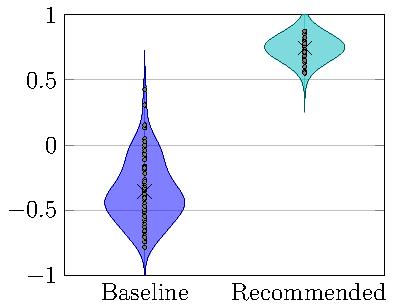
\includegraphics[width=.2\textwidth]{Figs/econ_cmp-figure3.pdf}}%
%         \label{subfig:econ_shap_spearmans}%
%       }\hspace{1cm}
%       \subfloat[SHAP Relevance]{%
%         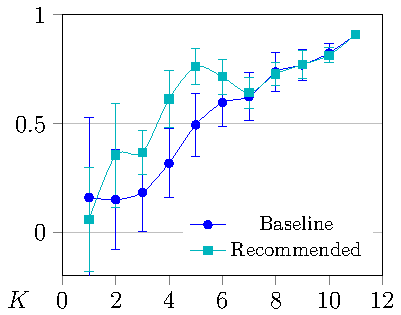
\includegraphics[width=.2\textwidth]{Figs/econ_cmp-figure5.pdf}%
%         \label{subfig:econ_shap_recalls}%
%       }\\
%       \subfloat[LIME Directionality]{%
%         \raisebox{.2cm}{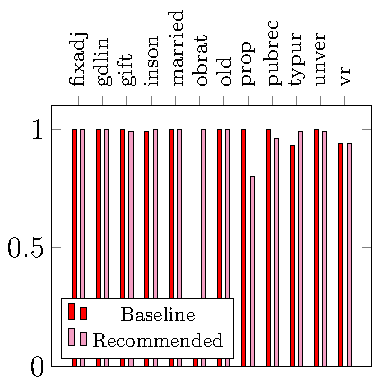
\includegraphics[width=.2\textwidth]{Figs/econ_cmp-figure0.pdf}}%
%         \label{subfig:econ_lime_sign_accs}%
%       }\hspace{1cm}
%       \subfloat[LIME Concordance]{%
%         \raisebox{.05cm}{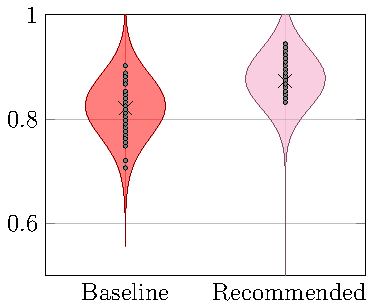
\includegraphics[width=.2\textwidth]{Figs/econ_cmp-figure2.pdf}}%
%         \label{subfig:econ_lime_spearmans}%
%       }\hspace{1cm}
%       \subfloat[LIME Relevance]{%
%         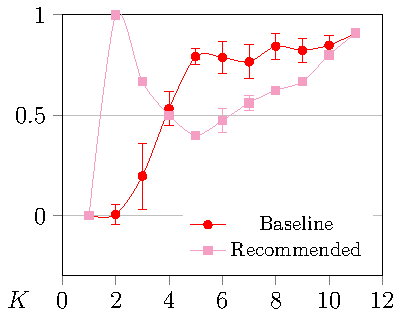
\includegraphics[width=.2\textwidth]{Figs/econ_cmp-figure4.pdf}%
%         \label{subfig:econ_lime_recalls}%
%       }\\
%       \caption{Improvements due to use of recommended pipeline instead of one without any of our mitigation strategies}\label{fig:econ_cmp}
%     \end{figure}
  

\vspace{-3mm}
\subsection{Case Study: Replicating Econometric Findings}
  \label{sec:case_study}\vspace{-3mm}
  To validate the efficacy of our mitigation strategies and illustrate how they could be employed in practice, we will compare how well two combined strategies reproduce insights from an econometric paper on the approval of home loan applications \citep{bane2006econometric} against default usage of SHAP and LIME. The home loan data set is publicly available and originates from a study by the Federal Reserve Bank of Boston \citep{hunter1996cultural}. We take the ground truth marginal effects $\boldsymbol{\beta}$ underlying this data set to be the coefficients of the logistic regression model obtained in the analysis of \cite{bane2006econometric}. 
  %%This is justifiable because econometric modeling is equipped to capture marginal effects. 
  The linear ground truth model derived from their logistic regression model appears in Equation \ref{eqn:econ_gt}. 
  %%The meanings and ranges of each feature appear in Appendix Table \ref{tab:case_study_features}. %We will use the logistic regression coefficients to evaluate SHAP and LIME explanations in the same manner as has been done throughout this paper. We suppose that the logistic regression coefficients have the correct signs and magnitudes relative to each other, not that the logistic regression itself is the true causal model underlying home loan approvals in Boston. 

  %%Our two combined strategies are versions of the general strategy outlined in Section \ref{sec:summary_and_strategies} tailored to SHAP and LIME. 
  We developed combined mitigation strategies for both SHAP and LIME. The SHAP strategy is simply to normalize the SHAP values. The LIME strategy is to set average the explanations of 10 MLPs with AUC at least $.9$ given by 10 LIME explainers with $\nu=n=10000$ and differing random seeds. We test these strategies against individual SHAP and LIME explainers using default settings.
  %%We will perform the following comparison to evaluate them. First, we split the data set into 80\% training data and 20\% testing data. Then we train 10 MLPs with test set AUC that are all near $.92$. The LIME variant of the strategy uses all $B=10$ MLPs and $E=10$ LIME explainers for each MLP. Each LIME explainer has $\nu=n=10000$. Because SHAP is (essentially) deterministic and the MLP averaging strategy did not significantly increase directionality and concordance for SHAP, we use $B=E=1$ and normalize the Shapley values. Baseline explanations come from explanations of one MLP with accuracy $.86$, ROC AUC $.93$ with individual SHAP and LIME explainers both using default settings. 
  %\begin{tcolorbox}[title = Econometric Ground Truth Model $\mathcal{G}$]
  \vspace{-3mm}
  \begin{eqnarray}
  \label{eqn:econ_gt}
  \small
    \mathcal{G}(X) =.8 + 3.5\cdot \text{good credit} + 4.7\cdot \text{purchaser type} -4.4 \cdot \text{PMI approved} - .4 \cdot \text{multi family} -2.5 \cdot \text{unver} + \nonumber \\ .9 \cdot \text{fixed rate} - 1.4 \cdot \text{bankruptcy} - .9 \cdot \text{value rate} - .03 \cdot \text{debt rate} - .7 \cdot \text{old} + .8 \cdot \text{married} - .8 \cdot \text{gift}\vspace{-3mm}
  \end{eqnarray}
  %\end{tcolorbox}
  %\subsection{Baseline Performance}
  %Figure \ref{fig:econ_cmp} compares the explanation quality for 100 applicants from the baseline pipeline and recommended pipeline. %In the Appendix, we show also compare results for importance sign accuracy, Spearman rank correlation, and recall.
We evaluate SHAP and LIME explanations before and after applying the strategies, comparing them against the ground truth $\boldsymbol{\beta}$. The overall results are shown in Figure \ref{fig:econ_cmp}
  Both the SHAP and LIME variants of our general strategy generally had results which improved upon the relevant baseline in at least one respect.% Using our mitigations with LIME significantly improved concordance overall, significantly improved directionality for ``fixed rate" and ``old", significantly improved relevance for the top $k=2,3$ features. %%It had significantly worse directionality only for ``vr" and ``obrat", and significantly worse relevance for features not in the top-4. 
It can be seen in Figure \ref{subfig:econ_shap_sign_accs} that our mitigated SHAP strategy significantly improved directionality for all features except ``good credit" (labeled as ``gdlin'') and ``multi family" (labeled as ``prop"). Figure \ref{subfig:econ_shap_spearmans} shows a great increase in concordance for SHAP, as the mean concordance of applicants' rankings went up from about $-.36$ to about $.45$. Additionally, Figure \ref{subfig:econ_shap_recalls} shows great gains in relevance for all $k\neq 1,11$. We observed similar improvement in the three metrics for LIME, too. %As for LIME, Figure \ref{subfig:econ_lime_sign_accs} shows that directionality was significantly improved just for ``fixed rate`` (labeled as ``fixadj". Figure \ref{subfig:econ_lime_spearmans} shows that our strategy improved concordance for LIME on average. Finally, Figure \ref{subfig:econ_lime_recalls} shows that relevance was significantly improved for LIME for $k=2,\ldots,5$. 
In spite of these improvements, however, the mitigated explanations were still imperfect and could not yield the same insights as the econometrics work we used as a reference.
  
%\textcolor{red}{1) talk about SHAP first 2) refer to the specific subplot when discussing the results in detail.  }

    % % econ
    % \begin{figure}[t!]
    %   \centering
    %   \subfloat[SHAP Directionality]{%
    %     \raisebox{.2cm}{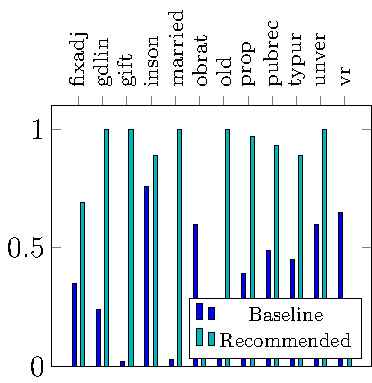
\includegraphics[width=.2\textwidth]{Figs/econ_cmp-figure1.pdf}}%
    %     \label{subfig:econ_shap_sign_accs}%
    %   }\hspace{1cm}
    %   \subfloat[SHAP Concordance]{%
    %     \raisebox{.05cm}{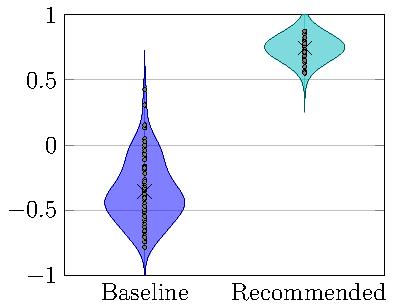
\includegraphics[width=.2\textwidth]{Figs/econ_cmp-figure3.pdf}}%
    %     \label{subfig:econ_shap_spearmans}%
    %   }\hspace{1cm}
    %   \subfloat[SHAP Relevance]{%
    %     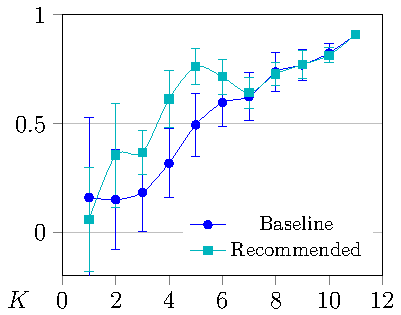
\includegraphics[width=.2\textwidth]{Figs/econ_cmp-figure5.pdf}%
    %     \label{subfig:econ_shap_recalls}%
    %   }\\
    %   \subfloat[LIME Directionality]{%
    %     \raisebox{.2cm}{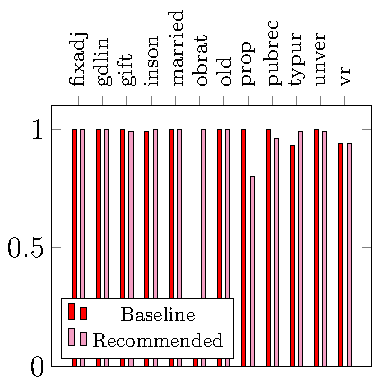
\includegraphics[width=.2\textwidth]{Figs/econ_cmp-figure0.pdf}}%
    %     \label{subfig:econ_lime_sign_accs}%
    %   }\hspace{1cm}
    %   \subfloat[LIME Concordance]{%
    %     \raisebox{.05cm}{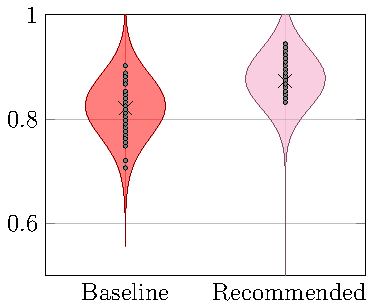
\includegraphics[width=.2\textwidth]{Figs/econ_cmp-figure2.pdf}}%
    %     \label{subfig:econ_lime_spearmans}%
    %   }\hspace{1cm}
    %   \subfloat[LIME Relevance]{%
    %     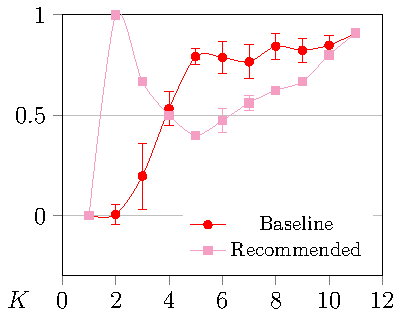
\includegraphics[width=.2\textwidth]{Figs/econ_cmp-figure4.pdf}%
    %     \label{subfig:econ_lime_recalls}%
    %   }\\
    %   \caption{Improvements due to use of recommended pipeline instead of one without any of our mitigation strategies}\label{fig:econ_cmp}
    % \end{figure}
  
\vspace{-3mm}\section{Discussion and Conclusion}
  \label{sec:discussion}\vspace{-3mm}
  As post hoc explanations gain popularity in business research, we have identified an alarming trend of using them to make claims about the underlying variable relationships in the data. In our survey of 150 business papers, we found that 42\% of them use LIME or SHAP for this purpose. The validity of this use of post hoc explanations has not been studied in the literature, making this paper the first effort towards this purpose. In the following sections, we will summarize our findings and discuss the general use of post hoc explainers in business research.
  %  
  %In this paper we have introduced and investigated issues of misalignment and inconsistency of post hoc explanations. Our thorough literature review uncovered that business researchers using post hoc explanations value data-alignment. Thus we have contributed to the business literature by providing both theoretical and empirical evidence that the two most popular explainers, LIME and SHAP, often produce misaligned explanations. Notably, we proved that SHAP is inherently unsuitable to infer information about $\boldsymbol{\beta}$. %We have also identified various factors that contribute to misalignment and inconsistency. 
  %We also contribute to the business literature by proposing some simple and intuitive mitigation strategies which we found to benefit explainer data-alignment to varying extents.

\vspace{-3mm}
  \subsection{Main Findings}\vspace{-3mm}
    Our paper contributes several important findings to the use of post hoc explanations in business research.


    %%The way in which authors use SHAP and LIME shows that they implicitly value data-alignment. There is also a growing number of papers that recommend explaining ML models with SHAP instead of using traditional econometric methods like Ordinary Least Squares (OLS). The underlying rationale is that machine learning models are better equipped to process large numbers of features, need comparatively feature engineering, and can capture feature interactions. 
     First, through an extensive literature review, we found that the use of post hoc explanations to infer information about the data is quite prevalent. In the 150 papers we reviewed, 63 used SHAP or LIME to draw conclusions about the $X\rightarrow Y$ relationship instead of the $\mathcal{M}(X)\rightarrow Y$ relationship. Such use deviates from the intended purpose of post hoc explainers: they are designed to explain the machine learning model, not to infer any information from the data. Identifying this misuse of post hoc explanations is an important contribution of this paper. Note that while post hoc explanations have been first introduced and widely used in the machine learning community, the issue we discuss in this paper is less of a concern for that community because computer scientists are more interested in model explanations. Post hoc explainers are used to understand a machine learning model's behavior in order to diagnose and debug the model. However, social scientists and business researchers try to understand the data and the underlying phenomena, making this issue more prominent in business research.


    Second, we provide both theoretical and empirical evidence that SHAP and LIME explanations are, in fact, not data-aligned. In our investigation, we discovered that SHAP and LIME incorrectly represent the signs and relative importance of the marginal effects of the explanatory variables used to train the models they explain. As shown in Section \ref{sec:causes_of_misalignment}, SHAP and LIME tend to be data-misaligned even in scenarios where they explain an accurate machine learning model trained on data whose features are mutually independent and whose target is derived from a simple linear ground truth model (scenarios which are, in a sense, ideal).%This observation suggests a need for caution when interpreting variable relationships based on post hoc explanations.
    %%It opens up a dialogue about the complexities of deriving accurate insights from such models, contributing to a deeper understanding of their limitations and paving the way for future research in this area. In light of these insights, it may be beneficial for the academic community to revisit prior analyses that have relied heavily on post hoc explanations. This reassessment could ensure that interpretations and conclusions drawn from such models are robust and reflective of their underlying dynamics. Our findings underscore the importance of continuous critical evaluation in the field, especially as we seek to refine our understanding and application of these explanatory tools. %Our finding is echoed in other recent studies that compared the \cite{baghdasaryan2021comparison}
    
Third, we identify factors that contribute to data-misalignment. The designs of SHAP and LIME naturally lead to misalignment because the coefficients they produce are, in general, not the marginal effects of the prediction function being explained. More specifically, we show that the design of SHAP naturally lends itself to misalignment because Shapley values differ from marginal effects. LIME's use of weighted ridge regression on discretized features, as opposed to OLS, prevents it from exactly recovering marginal effects. We also identified that the predictive performance of the black box model, the independence of the features, and the dimensionality of the training data are factors external to the explainers that are associated with misalignment. Our experiments demonstrated that explanations of models with lower predictive performance and explanations of models trained on datasets that were not relatively low dimensional and with mutually independent features tended to be less data-aligned. %\textcolor{red}{talk about 1) explainer-specific reasons and 2)general reasons } that the reason for the data-alignment is different for SHAP and LIME. %Achieving data-alignment using unmodified SHAP feature importance values is inherently impossible due to the nature of Shapley values.
    %%Shapley values represent a feature's contribution to a prediction by considering not only the feature's marginal effect but also its value and the influence of other variables within the explanation process. In the particular case where SHAP explains a linear model, the vector of Shapley values is given by $\boldsymbol{\beta}(\boldsymbol{\xi}-\bar{\mathbf{x}})$, diverging from a direct representation of $\boldsymbol{\beta}$. 
    %Conversely, LIME's data-alignment arises from the mechanics of its default ridge regression approach. 
    %%Our analysis, supported by Theorem \ref{thm:lime_thm}, indicates that LIME could achieve data-alignment by avoiding the discretization of numerical inputs, sampling many points for its synthetic regression problem, and opting for a significantly larger bandwidth than the default. Yet, even with these adjustments, common properties of real-world data such as correlated variables often hinder the attainment of data-alignment. Nonetheless, it is noteworthy that our evaluations generally reveal \textit{LIME to provide explanations of higher concordance and relevance compared to SHAP}.
 
    
  Finally, we identify several mitigation strategies that show promise in enhancing the data-alignment of explanations across various stages of the explanation pipeline. These strategies, validated through empirical testing, offer significant improvements in aligning explanations more closely with marginal effects. However, it is important to acknowledge that none of the strategies can guarantee complete congruence with marginal effects. This absence of a full guarantee means that while explanations may sometimes align closely with the marginal effects, they cannot reliably do so, thus calling for great caution when researchers use them. %the lack of certainty could pose challenges for their adoption.
    %%Such a scenario potentially restricts the applicability of post hoc explanations, as users may remain uncertain about the extent to which these explanations accurately mirror the underlying the marginal effect structure. This limitation underscores the need for cautious interpretation and application of post hoc explanation methods in practical scenarios.
  
\vspace{-3mm}  \subsection{On the Use of Post Hoc Explanations}\vspace{-3mm}
  We want to emphasize that this paper focuses on the issue of using post hoc explanations to make inferences about the ground truth information in $\mG$ that generates the data. We do not explore their use in explaining the machine learning model $\mM$ or its predictions $\mathcal{M}(X)$, which is the primary intended purpose of post hoc explainers. However, it is important to note that even this intended use of post hoc explainers raises some concerns \citep{garreau2020looking,alvarez18robustness,kumar20shap,jacovi2023diagnosing}. For the scope of this paper, our discussion is solely focused on inferring ground truth information from $\mathcal{G}$ through the explanations for $\mathcal{M}$.
\vspace{-3mm}
  \paragraph{General Usage}
  While this paper recommends against using post hoc explanations to make any definite claims about marginal effects, it does not mean that post hoc explanations cannot be used at all. Instead of using them as a tool to \textbf{validate} hypotheses and viewing the explanations as evidence, we propose to use post hoc explanations to \textbf{propose} hypotheses that can guide subsequent efforts after they are corroborated. 
  %%As a preliminary step, researchers can use the level of inconsistency between explanations of models trained on different splits of the data to gauge data-alignment, viewing explanations which do not share common patterns found the collection of explanations as an indication of its implausibility. Following the preliminary step,
   As was done in \cite{tang2024china}, plausible post hoc explanations can also be used to aid classical regression analyses as a feature selection method. That is, researchers can opt to use only those features which are said to be important by a post hoc explainer(s) in their regressions but should keep in mind that those features may not actually be important to $\mathcal{G}$. Another theme of usage is to leverage both SHAP and another method which is more suitable for causal identification in deriving conclusions. For example,  \cite{zhang2023can} follows up their search for important features for restaurant survival using SHAP by using causal forests to estimate the treatment effects of those features. Similarly, \cite{hanauer22boosting} use traditional regression as a trusted baseline that they compare SHAP explanations to. 


\vspace{-3mm}\subsection{Final Remarks}\vspace{-3mm}% and Future Work}
This paper aims to highlight the issue with a use of post hoc explanations that we identify as inappropriate. To demonstrate the seriousness of this problem, we show that it occurs even in the simplest context, where the ground truth $\mathcal{G}$ is linear. Even in this simple case, SHAP and LIME produce misaligned explanations. We expect that in more realistic scenarios their performance can only be worse. Real decision processes are often non-linear and involve feature interactions and unobservable features; naturally, these added complexities should reduce the efficacy of SHAP and LIME, making it even more challenging to obtain data-aligned explanations. Given the uncertainty regarding the validity of post hoc explanations, researchers should view them skeptically and consider them as hypotheses rather than definitive claims about reality.



% References here (outcomment the appropriate case)

% CASE 1: BiBTeX used to constantly update the references
%  (while the paper is being written).
%\bibliographystyle{informs2014} % outcomment this and next line in Case 1
%\bibliography{<your bib file(s)>} % if more than one, comma separated

% CASE 2: BiBTeX used to generate mypaper.bbl (to be further fine tuned)
%\input{mypaper.bbl} % outcomment this line in Case 2

%If you don't use BiBTex, you can manually itemize references as shown below.

\pagebreak


\bibliographystyle{informs2014}
\bibliography{refs}

   % pipeline
   \begin{figure}[ht!]
    \centering
    \captionsetup{labelfont=footnotesize,textfont=footnotesize}
    %\fbox{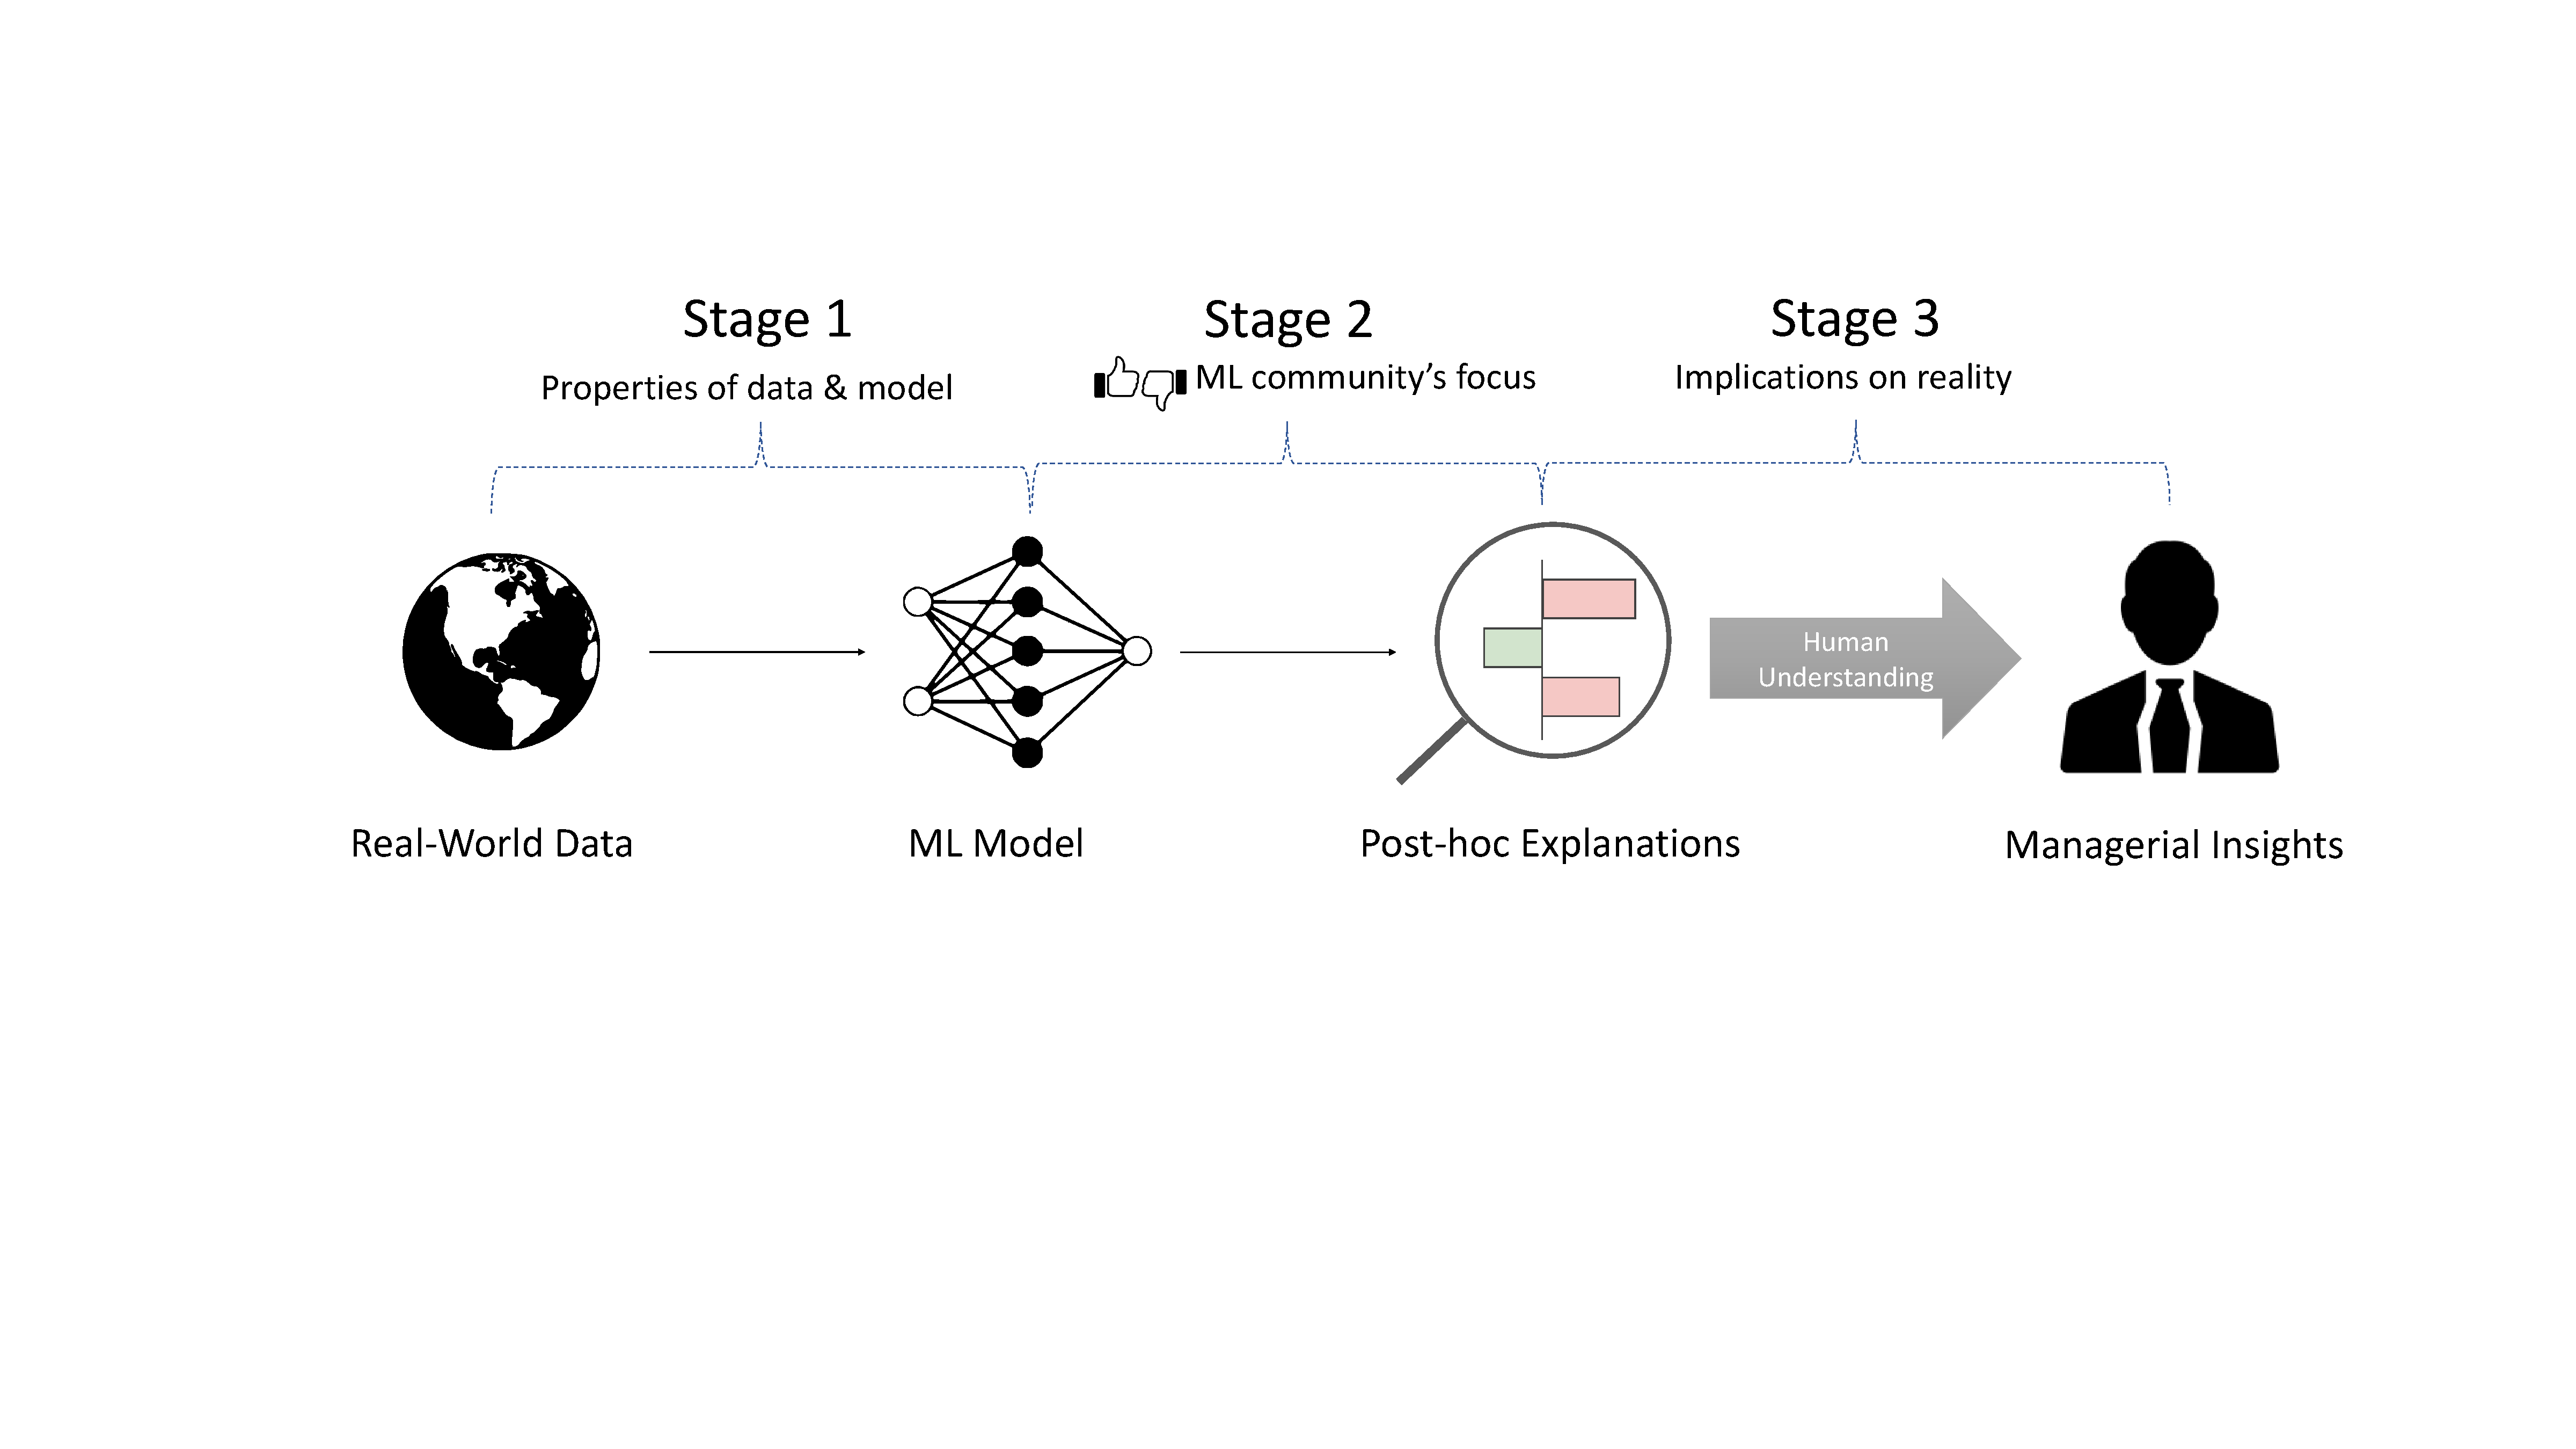
\includegraphics[width = \textwidth,trim=250 500 150 250 mm, clip=true]{Figures/pipeline.pdf}}
    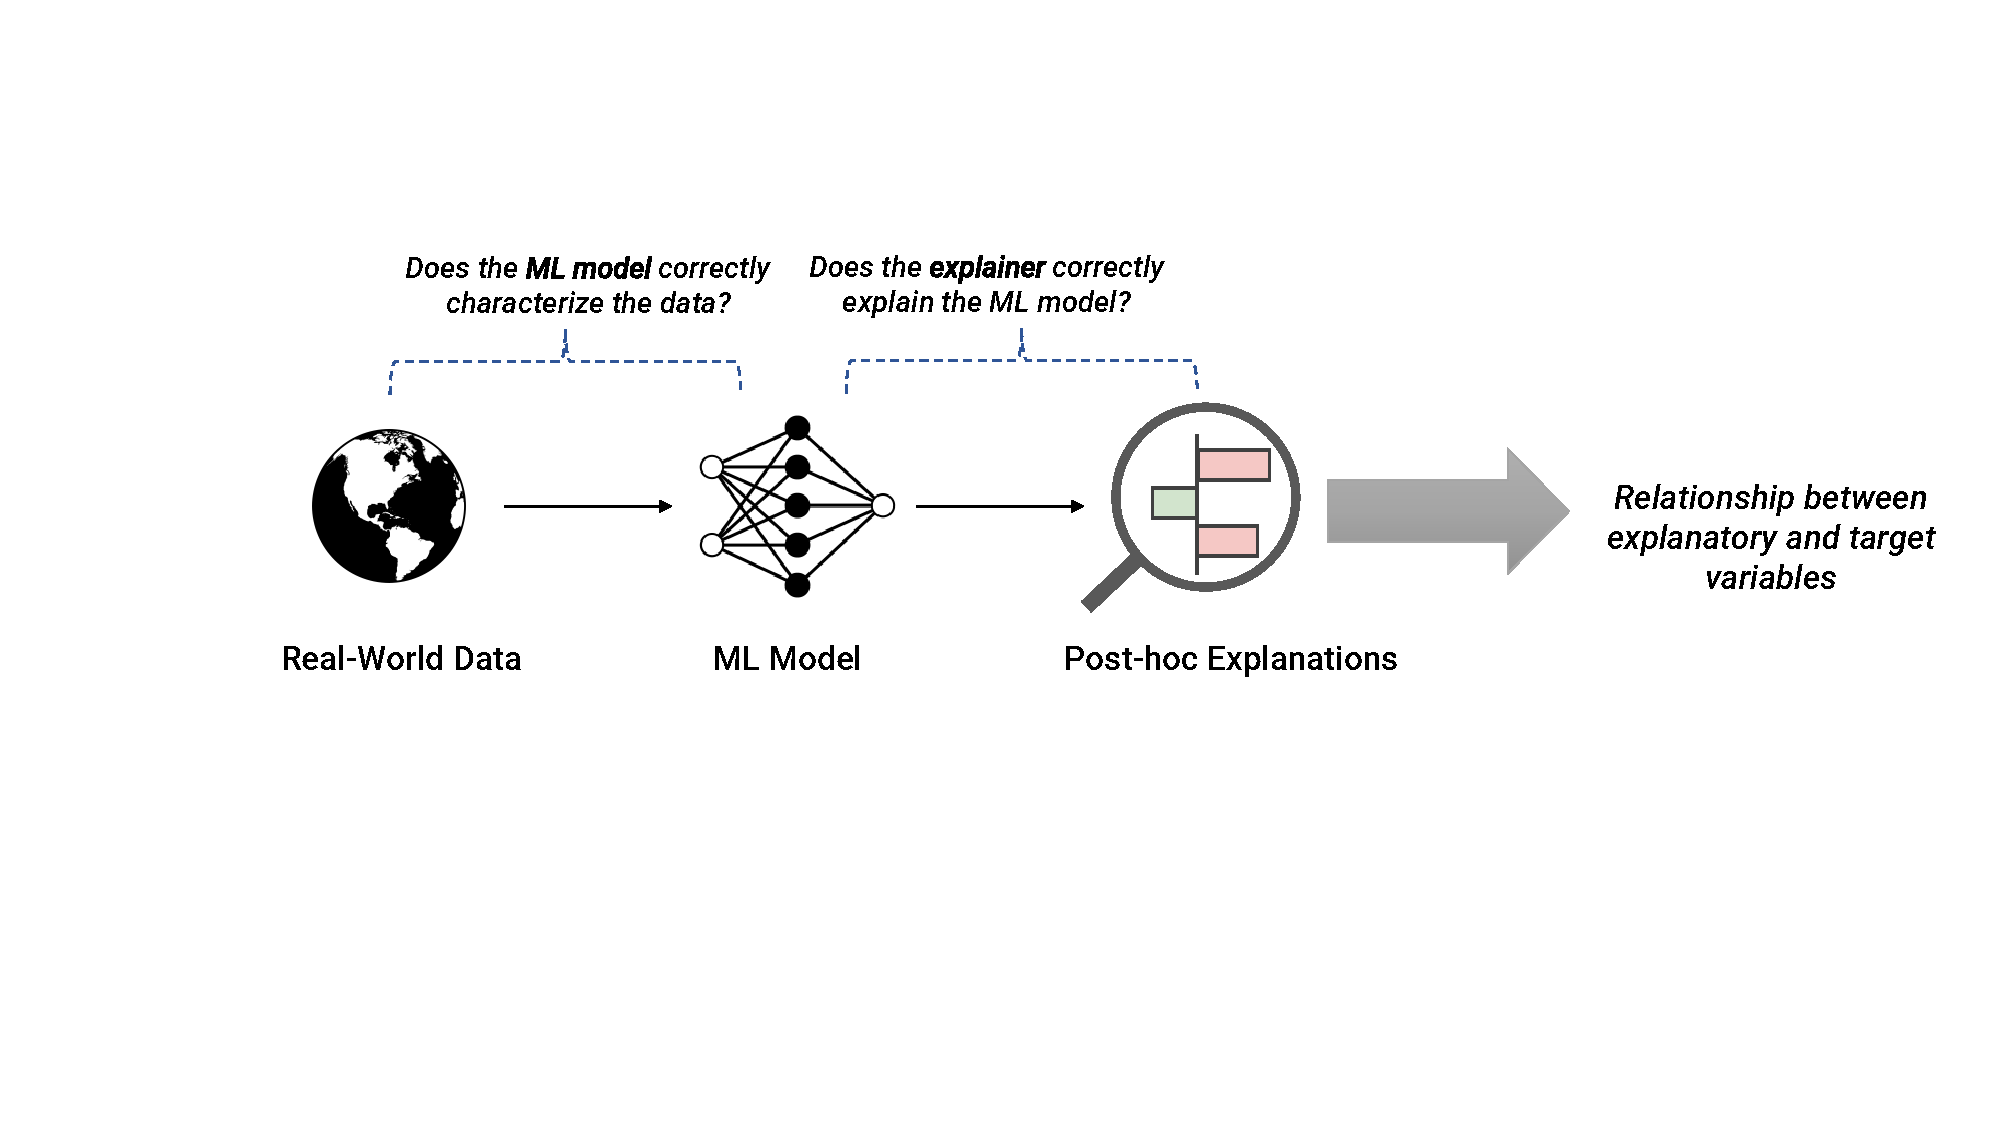
\includegraphics[trim={4.75cm 7.5cm 1.125cm 4.25cm},clip,width = 0.8\textwidth]{Figures/pipeline_flow_new.pdf}
    \caption{Explanation Pipeline: the pipeline of using post hoc explainers to explain a machine learning model. Inferring information about the actual marginal effects of the features constitutes mistaken usage of the pipeline.}
    \label{fig:pipeline}
  \end{figure}



    % auc and colinear
    \begin{figure}[ht!]
    \centering
    \captionsetup{labelfont=footnotesize,textfont=footnotesize}
    \begin{minipage}{.475\textwidth}
     \centering
     \captionsetup[subfloat]{labelfont=scriptsize,textfont=scriptsize}
      \subfloat[SHAP Directionality]{
        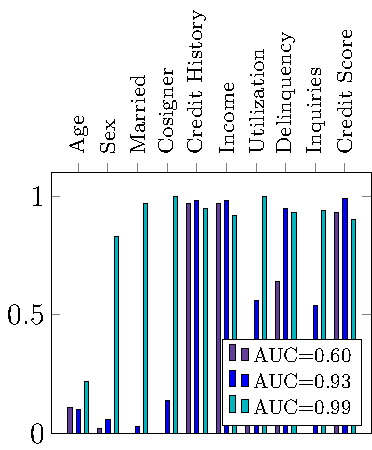
\includegraphics[width=.375\textwidth]{Figs/sec4_4_mlp_auc_shap-figure0.pdf}
        \label{subfig:mlp_auc_shap_sign_accs}
      }\hspace{.1cm}
      \subfloat[LIME Directionality]{
        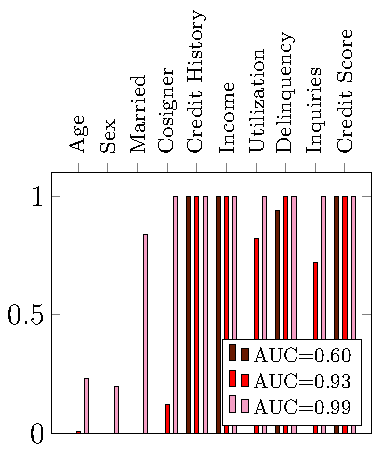
\includegraphics[width=.375\textwidth]{Figs/sec4_4_mlp_auc_lime-figure0.pdf}
        \label{subfig:mlp_auc_lime_sign_accs}
      } \\
      \subfloat[SHAP Concordance]{
        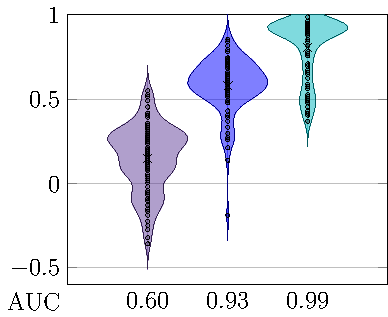
\includegraphics[width=.375\textwidth]{Figs/sec4_4_mlp_auc_shap-figure1.pdf}
      }\hspace{.1cm}
      \subfloat[LIME Concordance]{
        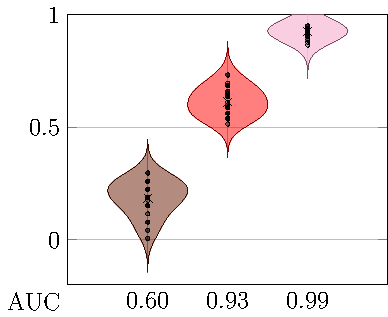
\includegraphics[width=.375\textwidth]{Figs/sec4_4_mlp_auc_lime-figure1.pdf}
      } \\
      \subfloat[SHAP Relevance]{
        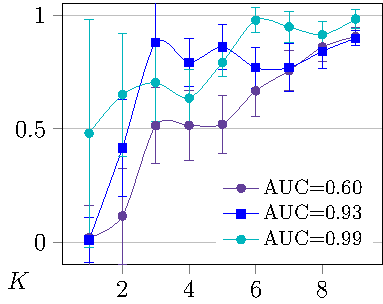
\includegraphics[width=.375\textwidth]{Figs/sec4_4_mlp_auc_shap-figure2.pdf}%
        \label{subfig:mlp_auc_shap_recalls}
      }\hspace{.1cm}
      \subfloat[LIME Relevance]{
        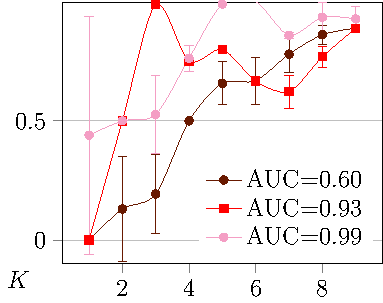
\includegraphics[width=.375\textwidth]{Figs/sec4_4_mlp_auc_lime-figure2.pdf}%
        \label{subfig:mlp_auc_lime_recalls}
      } 
      \label{fig:mlp_auc_increase}
      \caption{Comparisons of results for our three metrics for SHAP and LIME when explaining models with increasing predictive performance}%$\mathcal{M}_1$ with AUC=.6, $\mathcal{M}_2$ with AUC=0.92, and $\mathcal{M}_3$ with AUC=.99}
      \label{fig:mlp_auc_increase}
    \end{minipage}%
    \hspace{.1cm}
    \begin{minipage}{.475\textwidth}
     \centering
     \captionsetup[subfloat]{labelfont=scriptsize,textfont=scriptsize}
      \subfloat[SHAP Directionality]{
        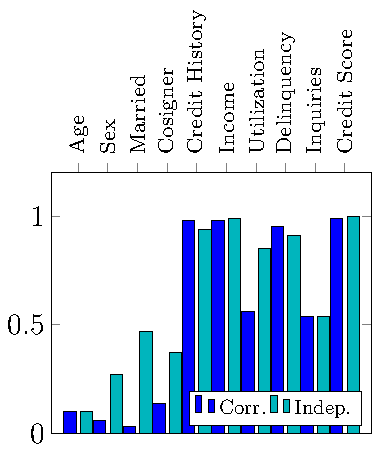
\includegraphics[width=.375\textwidth]{Figs/sec4_3_corr-figure1.pdf}
      }\hspace{.1cm}
      \subfloat[LIME Directionality]{
        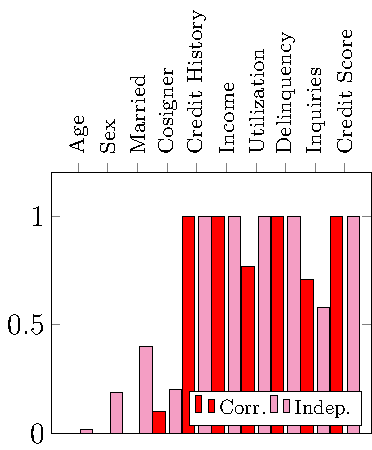
\includegraphics[width=.375\textwidth]{Figs/sec4_3_corr-figure0.pdf}
      } \\
      \subfloat[SHAP Concordance]{
        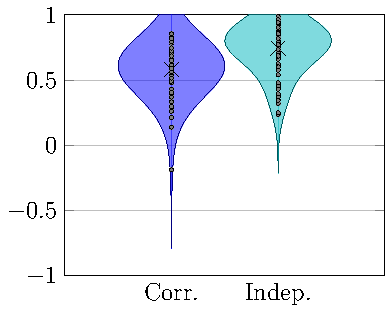
\includegraphics[width=.375\textwidth]{Figs/sec4_3_corr-figure3.pdf}
      }\hspace{.1cm}
      \subfloat[LIME Concordance]{
        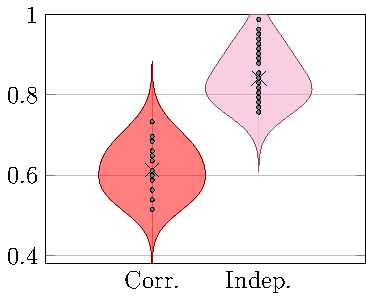
\includegraphics[width=.375\textwidth]{Figs/sec4_3_corr-figure2.pdf}
      } \\
      \subfloat[SHAP Relevance]{
        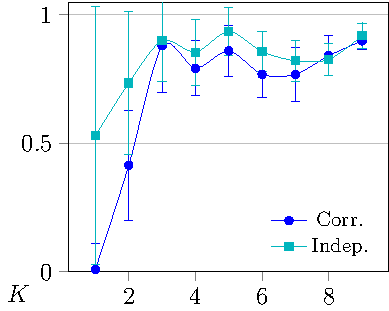
\includegraphics[width=.375\textwidth]{Figs/sec4_3_corr-figure5.pdf}
      }\hspace{.1cm}
      \subfloat[LIME Relevance]{
        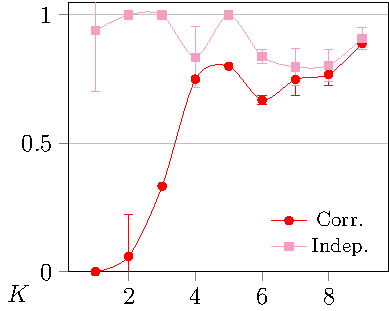
\includegraphics[width=.375\textwidth]{Figs/sec4_3_corr-figure4.pdf}
      } 
      \caption{Comparison of faithfulness of explanations of models trained on data with independent features versus data with two strongly correlated features}
      \label{fig:lime_shap_colinear}
    \end{minipage}
    \end{figure}

    % feature description table
\begin{table}[ht!]
\centering
\captionsetup{labelfont=footnotesize,textfont=footnotesize}
%\resizebox{\textwidth}{!}{%
\scriptsize
\begin{tabular}{c|c|c}
\toprule
\textsc{Feature} & \textsc{Explanation}              & \textsc{Formula}    \\ \toprule
Age       & Applicant Age                  & Uniform(18,100)    \\ 
Sex       & Applicant Sex                  & Bernoulli(.5)     \\
Married     & Applicant Marital Status            & Bernoulli(.5)     \\ 
Income      & Applicant Income                & Normal(40,000, 30,000) \\ 
Inquiries    & Number of credit inquiries           & Uniform(0,6)      \\ 
Cosigner     & Indicator of presence of loan cosigner & Function of marital status     \\ 
Utilization   & Proportion of total credit utilized      & Uniform(0,1)      \\ 
Delinquencies  & Number of delinquent payments in last 2 years & Uniform(0,24)     \\ 
Credit Score   & Credit score based on FICO scoring & FICO credit scoring model \citep{ligons_fico}      \\ \bottomrule
\end{tabular}%
%}
\caption{Description of features for simulated loan data.}
\label{tab:simulated}
\end{table}

    % pervasiveness
    \begin{figure}[ht!]
      \captionsetup{labelfont=footnotesize,textfont=footnotesize}
      \captionsetup[subfloat]{labelfont=scriptsize,textfont=scriptsize,justification=centering}
      \centering
      \subfloat[SHAP Mean Directionality]{%
        \hspace{0mm}
        \raisebox{0cm}{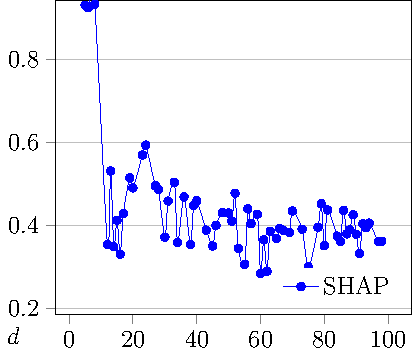
\includegraphics[width=0.178125\textwidth]{SynthFigs/meanaccshap-figure0.pdf}\quad}%
        \label{fig:shap_vary_d_spearmans}%
      }\hspace{1cm}%\hfill
      \subfloat[SHAP Concordance]{%
        \raisebox{0cm}{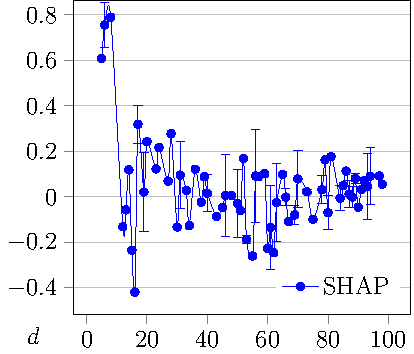
\includegraphics[width=0.178125\textwidth]{SynthFigs/concshap-figure0.pdf}}%
        \label{fig:shap_vary_d_accs}%
      }\hspace{1cm}%\hfill
      \subfloat[SHAP Top-3 Relevance]{%
        \raisebox{0cm}{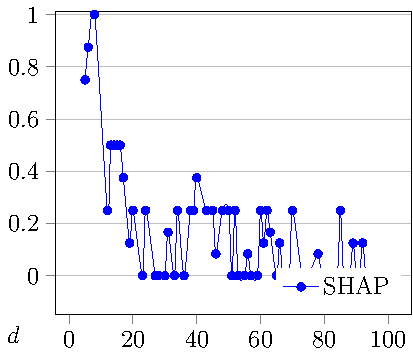
\includegraphics[width=0.178125\textwidth]{SynthFigs/relshap-figure0.pdf}}%
        \label{fig:shap_vary_d_spearmans}%
      }\\
      % \subfloat[LIME Top-1 Directionality]{%
      %   \raisebox{0cm}{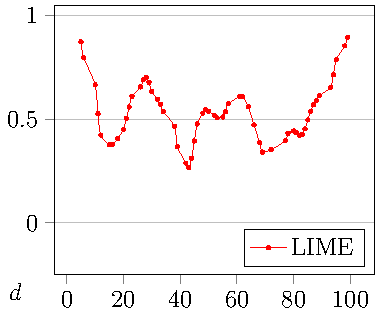
\includegraphics[width=.2\textwidth]{Figs/synthetic-figure1.pdf}}%
      %   \label{fig:lime_vary_d_accs}%
      % }\hspace{.5cm}%\hfill
      \subfloat[LIME Mean Directionality]{%
        \hspace{0mm}
        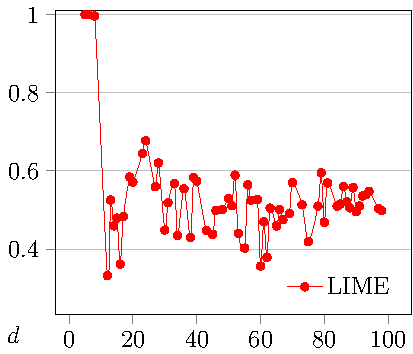
\includegraphics[width=0.178125\textwidth]{SynthFigs/meanacclime-figure0.pdf}\quad%
        \label{fig:lime_vary_d_spearmans}%
      }\hspace{1cm}%\hfill
      \subfloat[LIME Concordance]{%
        \hspace{0mm}
        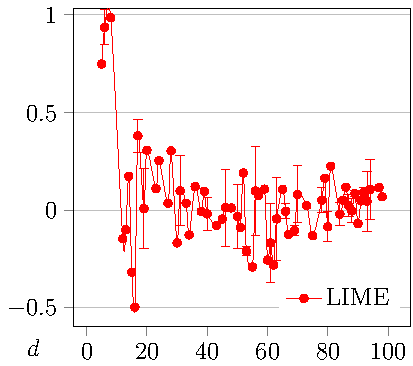
\includegraphics[width=0.178125\textwidth]{SynthFigs/conclime-figure0.pdf}%
        \label{fig:lime_vary_d_accs}%
      }\hspace{1cm}%\hfill
      \subfloat[LIME Top-3 Relevance]{%
        \hspace{0mm}
        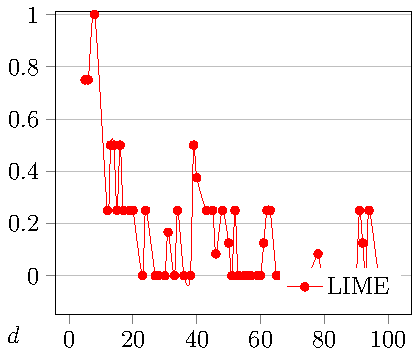
\includegraphics[width=0.178125\textwidth]{SynthFigs/rellime-figure0.pdf}%
        \label{fig:lime_vary_d_spearmans}%
      }\\
      \caption{Relationship of number of features $d$ with feature-wise mean directionality, concordance, and relevance for $k=3$}
      \label{fig:lime_shap_vary_d}
    \end{figure}

    % econ
    \begin{figure}[t!]
      \captionsetup{labelfont=footnotesize,textfont=footnotesize}
      \captionsetup[subfloat]{labelfont=footnotesize,textfont=footnotesize}
      \centering
      \subfloat[SHAP Directionality]{%
        \raisebox{.2cm}{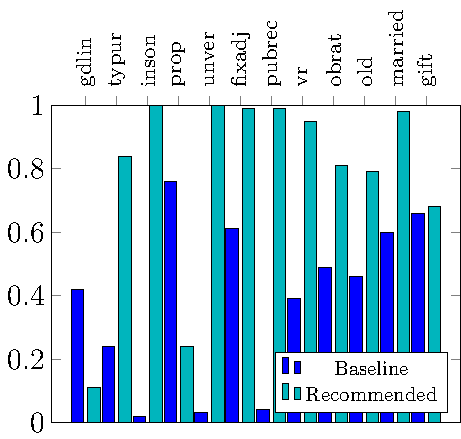
\includegraphics[width=.2\textwidth]{EconFigs/shap_econ-figure0.pdf}}%
        \label{subfig:econ_shap_sign_accs}%
      }\hspace{1cm}
      \subfloat[SHAP Concordance]{%
        \raisebox{.05cm}{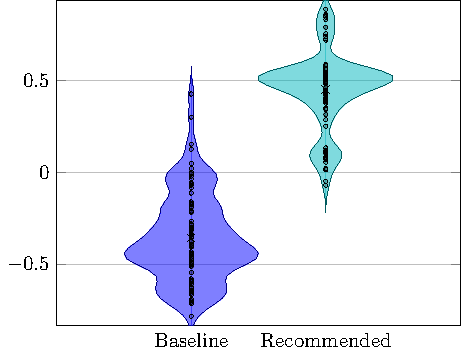
\includegraphics[width=.2\textwidth]{EconFigs/shap_econ-figure1.pdf}}%
        \label{subfig:econ_shap_spearmans}%
      }\hspace{1cm}
      \subfloat[SHAP Relevance]{%
        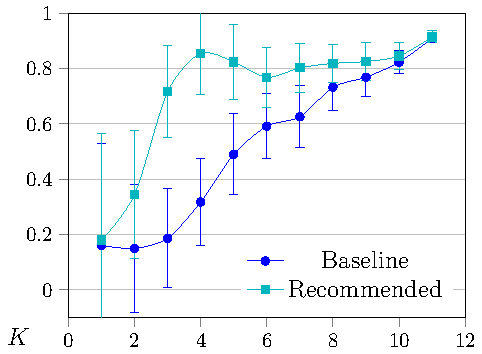
\includegraphics[width=.2\textwidth]{EconFigs/shap_econ-figure2.pdf}%
        \label{subfig:econ_shap_recalls}%
      }\\
      \subfloat[LIME Directionality]{%
        \raisebox{.2cm}{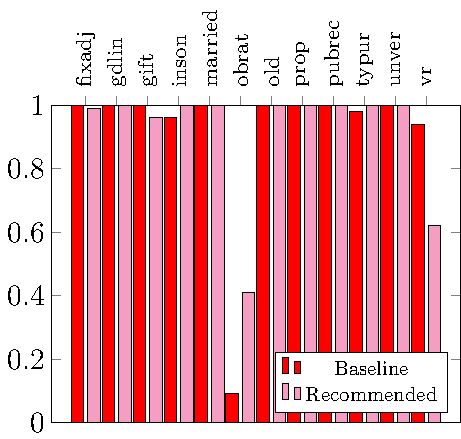
\includegraphics[width=.2\textwidth]{EconFigs/lime_econ-figure0.pdf}}%
        \label{subfig:econ_lime_sign_accs}%
      }\hspace{1cm}
      \subfloat[LIME Concordance]{%
        \raisebox{.05cm}{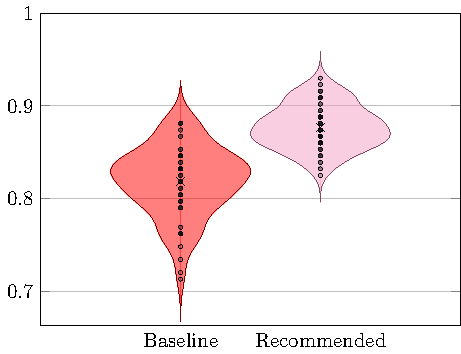
\includegraphics[width=.2\textwidth]{EconFigs/lime_econ-figure1.pdf}}%
        \label{subfig:econ_lime_spearmans}%
      }\hspace{1cm}
      \subfloat[LIME Relevance]{%
        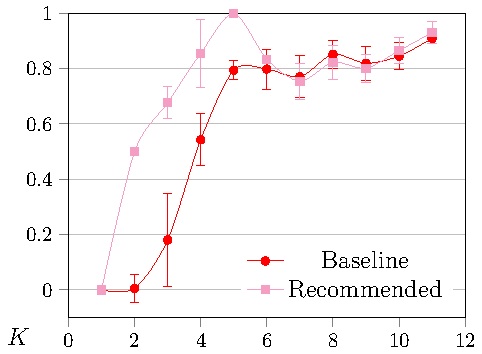
\includegraphics[width=.2\textwidth]{EconFigs/lime_econ-figure2.pdf}%
        \label{subfig:econ_lime_recalls}%
      }\\
      \caption{Improvements due to use of recommended pipeline instead of one without any of our mitigation strategies}\label{fig:econ_cmp}
    \end{figure}
  

% dimensions finds only 206 but indexes preprints%%%%%%%%%%%%%%%%%
\end{document}
%%%%%%%%%%%%%%%%%

